%!TEX root = ../../ClassicThesis.tex

In \autoref{ch:lam}, we considered the information about a naturalistic video stimulus contained in the power of oscillations in the \ac{CSD}.
In this chapter, we will investigate the information encoded in the phase of the \ac{CSD}, how this relates to the power or amplitude of the oscillations, and what properties of the stimulus may be encoded by the phase of the oscillations.


% =============================================================================
\section{Methods}
% =============================================================================

Since this dataset is the same as that analysed in \autoref{ch:lam}, the methodology for data collection and preprocessing are the same as were described in \autoref{sec:lam_exp}.


\subsection{Phase across depth and frequencies}
\label{sec:lam_phase_method}

The phase was computed in a similar manner to the power in \autoref{sec:lam_power_method}.
We filtered both the \ac{LFP} and \ac{CSD} using a series of bands each with a fractional bandwidth of $50\%$, spaced logarithmically at multiples of \num{1.291}.
This spacing ensures each band has $0\%$ overlap with bands further away than its immediate neighbours and a $44\%$ and $56\%$ overlap with its preceding and succeeding bands respectively.
The filter chosen was a zero-phase sixth-order Butterworth filter, after which the instantaneous phase was estimated by taking the angle of the Hilbert transform.
The phase in the \SIrange{4}{16}{Hz} and \SIrange{60}{170}{Hz} frequency bands was extracted in the same manner.


\subsection{Information contained in cortical oscillation phase}

The amount of information about the stimulus contained in the phase was computed in the same manner as the information in the power, described in \autoref{sec:lam_info_method}.
We again used \num{10} equipopulated bins, with the first bin starting at a phase of $0$ radians, and the final bin ending at $2\pi$ radians.
Due to the smooth, circular nature of phase, our samples of the phase vary uniformly across the range $[0, 2\pi)$ and hence the \num{10} bins each have a width of approximately $\nicefrac{\pi}{5}$ radians.

When computing the redundancy, we again used \num{3} equipopulated bins.
Hence for the phase, the bin widths were approximately $\nicefrac{2\pi}{3}$ radians.


\subsection{Signal and noise correlation}
\label{sec:pl_phase_correlation}

For both signal and noise correlation calculations, we used directional statistics (also known as circular statistics) which were were computed using the \textpackage{CircStat} toolbox \citep{Berens2009}.

The phase-phase correlations were evaluated with the circular-circular correlation coefficient \citep[page~176]{Jammalamadaka2001}, given by
\begin{equation}
% \rho_\text{CC}
% \rho_{\circlearrowleft \circlearrowleft}
\rho_{\circlearrowleft \circlearrowleft}(\alpha, \beta) = \frac{
\sum_{j = 1, \ldots, N} \, \sin(\alpha_j - \bar{\alpha}) \, \sin(\beta_j - \bar{\beta})
}{
\sqrt{\sum_{j = 1, \ldots, N} \, \sin^2(\alpha_j - \bar{\alpha}) \, \sin^2(\beta_j - \bar{\beta})}
},
\end{equation}
for $N$ samples of pairs of angles from distributions $\alpha$ and $\beta$, whose circular means are empirically determined to be $\bar\alpha$ and $\bar\beta$ respectively.

To find the phase-power correlations, we used the circular-linear correlation \citep[Equation~27.47]{Zar1998}, which is defined in terms of the linear-linear Pearson correlation coefficient, $\rho(X,Y)$, which we described in \autoref{eq:pearson}.
We define
$r_{sx} = \rho(\sin(\alpha), X)$,
$r_{cx} = \rho(\cos(\alpha), X)$, and
$r_{sc} = \rho(\sin(\alpha), \cos(\alpha))$
for a circular variable $\alpha$ and linear variable $X$, each using the Pearson correlation coefficient.
From this, the circular-linear correlation coefficient is given by
\begin{equation}
% \rho_\text{CL}
% \rho_{\circlearrowleft \nearrow}
\rho_{\circlearrowleft \rightarrow}(\alpha, X) = \sqrt{
\frac{
r_{sx}^2 + r_{cx}^2 - 2 \, r_{sx} \, r_{cx} \, r_{sc}
}{
1 - r_{sc}^2
}
}.
\end{equation}

To determine the statistical significance of our results, we also computed bootstrapped phase-phase and phase-power correlation coefficients.
We performed the correlation coefficient calculation with randomly paired $\alpha_j$ and $\beta_j$ values (for phase-phase) and $\alpha_j$ and $X_j$ values (for phase-power).
This was repeated for \num{20} shuffled copies of the time series data.%
\footnote{Which was shuffled after extracting phase and power values.}
After averaging over sessions, correlation coefficients which were less than three standard deviations of the bootstraps from the bootstrap mean were deemed not significantly correlated (shown in white in Figures \ref{fig:lam_noisesignal_corr_phase} and \ref{fig:lam_noisesignal_corr_depth}).


\subsection{Phase synchrony}

We defined the phase synchronization as the absolute magnitude of the vector average of the difference in phase \citep{Kreuz2011}.
Let us consider two random variables, $X$ and $Y$, whose phases, $\alpha$ and $\beta$ respectively, are simultaneously observed on $N$ occassions.
The vector average of the phase difference between $X$ and $Y$ is given by the complex number
\begin{equation}
z_{\alpha, \beta} = \frac{1}{N} \sum_{j = 1, \ldots, N} \exp(\iu (\alpha_j - \beta_j))
,\end{equation}
where $\iu$ is the imaginary unit, $\iu = \sqrt{-1}$.
From this, we determined the average phase difference as
\begin{equation}
\left<\Delta\phi\right> = \arg(z_{\alpha, \beta}) = \operatorname{atan2}(\Re(z_{\alpha, \beta}), \Im(z_{\alpha, \beta}))
,\end{equation}
and the phase synchrony as
\begin{equation}
R_{\alpha, \beta} = |z_{\alpha, \beta}| = \operatorname{abs}(z_{\alpha, \beta})
.\end{equation}


\subsection{Cross-frequency phase-amplitude coupling}
\label{sec:lam_cfc_method}

Strength of cross-frequency coupling was measured using the modulation index \citep{Tort2010}.
\ac{CSD} data was filtered for two bands, \SIrange{4}{16}{Hz} and \SIrange{60}{170}{Hz}, using a zero-phase sixth-order Butterworth filter, and the instantaneous phase of \SIrange{4}{16}{Hz} and envelope amplitude of \SIrange{60}{170}{Hz} were each estimated using a Hilbert transform.
We took a histogram of the \SIrange{4}{16}{Hz} phase datapoints with $M = 16$ bins each of width $\nicefrac{\pi}{8}$ radians, and for each bin took the average of the \SIrange{60}{170}{Hz} amplitudes simultaneously co-occurring with each of the phases in that bin.
This provides the expected amplitude, $a(j)$, at one depth as a function of phase, $\phi(j)$, at another depth, indexed by the bin index, $j$.

We then normalise $a$ against the total over all bins, $a'(j) = a(j) / \sum_k a(k)$,
such that $a'$ has the properties of a discrete probability density function.

Next, we utilise the \ac{KL} divergence, in general given by
\begin{equation}
D_\text{KL}(P \| Q) = \sum_k P(k) \log_2 \frac{P(k)}{Q(k)}
\end{equation}
for two discrete probability distributions $P$ and $Q$.
The \termemph{modulation index} is defined as the normalised \ac{KL} divergence of the distribution $a'$ from a uniform distribution \citep{Tort2010}, which is given by
\begin{equation}
\operatorname{MI} = \frac{
\log_2(M) + \sum_{j = 1,\ldots,M} a'_j \, \log_2(a'_j)
}{
\log_2(M)
}
.\end{equation}


% =============================================================================
\section{Results}
% =============================================================================


%-------------------------------------------------------------------------------
%\FloatBarrier
\subsection{Information contained in phase of cortical oscillations}

We computed the amount of information about the movie encoded in the phase of oscillations in both cortical \ac{LFP} and \ac{CSD}, as a function of cortical depth and oscillation frequency.
As shown in \autoref{fig:lam_phase_info}, we find that there is more information in the phase than the power of oscillations (see \autoref{fig:lam_info}) for all frequencies lower than \SI{40}{Hz}.
The phase contains much less information for higher frequencies, and the power contains more information than the phase for all frequencies above \SI{40}{Hz}.
Intuitively, this is because the phase of high frequency oscillations changes more rapidly and hence it is harder for it to be well aligned across trials than the phase of lower frequency oscillations.
In contrast, power of an oscillation fluctuates with the envelope amplitude of the oscillation, which can change much slower than the frequency of the oscillations.
Hence the power of fast oscillations can be stable enough to demonstrate repeatability across trials.

Similar to the results for power, we find that the phase of oscillations in the \ac{LFP} and \ac{CSD} produce similar results, but the \ac{CSD} provides superior spatial localisation (although the information in the \ac{CSD} is reduced compared with the \ac{LFP}).
For brevity, we therefore only consider the information in the \ac{CSD} for the remainder of the chapter.

\begin{figure}[htbp]
    \centering
    \hspace*{\fill}
    \subfloat[\ac{LFP} phase information.\label{fig:lam_phase_info_lfp}]{
        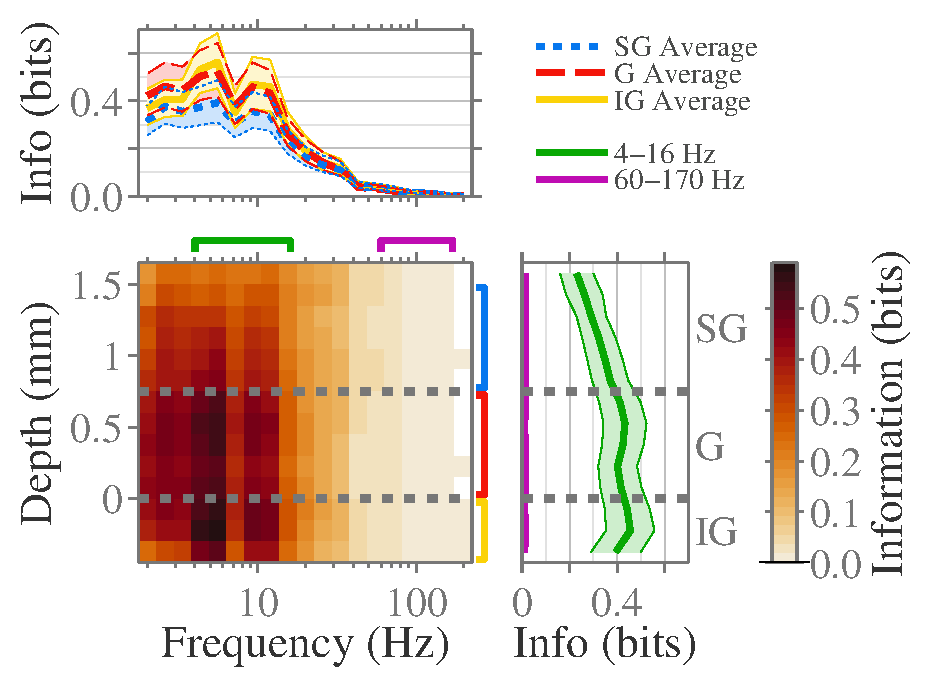
\includegraphics[scale=.45]{phaseinfo/fig3set-info-Cln-phase-straightnanmean-compzonescb-legend.eps}}
    \hspace*{\fill}\hspace{.2cm}\hspace*{\fill}
    \subfloat[\ac{CSD} phase information.\label{fig:lam_phase_info_csd}]{
        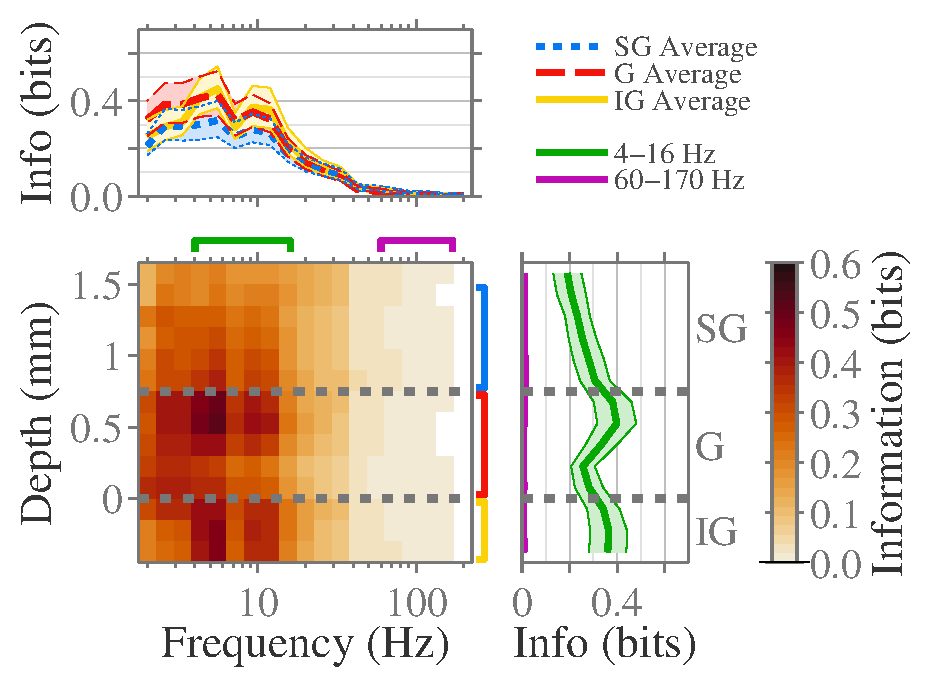
\includegraphics[scale=.45]{phaseinfo/fig3set-info-Csd-phase-straightnanmean-compzonescb-legend.eps}}
    \hspace*{\fill}
    \caption{
Information about the stimulus contained in the phase of the extracellular neural signal, as a function of frequency. Mean of 6 sessions.
\protect\subref{fig:lam_phase_info_lfp}:~\ac{LFP}.
\protect\subref{fig:lam_phase_info_csd}:~\ac{CSD}.
}
\label{fig:lam_phase_info}
\end{figure}

% \begin{figure}[htbp]
%     \centering
%     \hspace*{\fill}
%     \subfloat[\sesname{H05391}\label{fig:lam_phase_info_lfp_H05391}]{
%         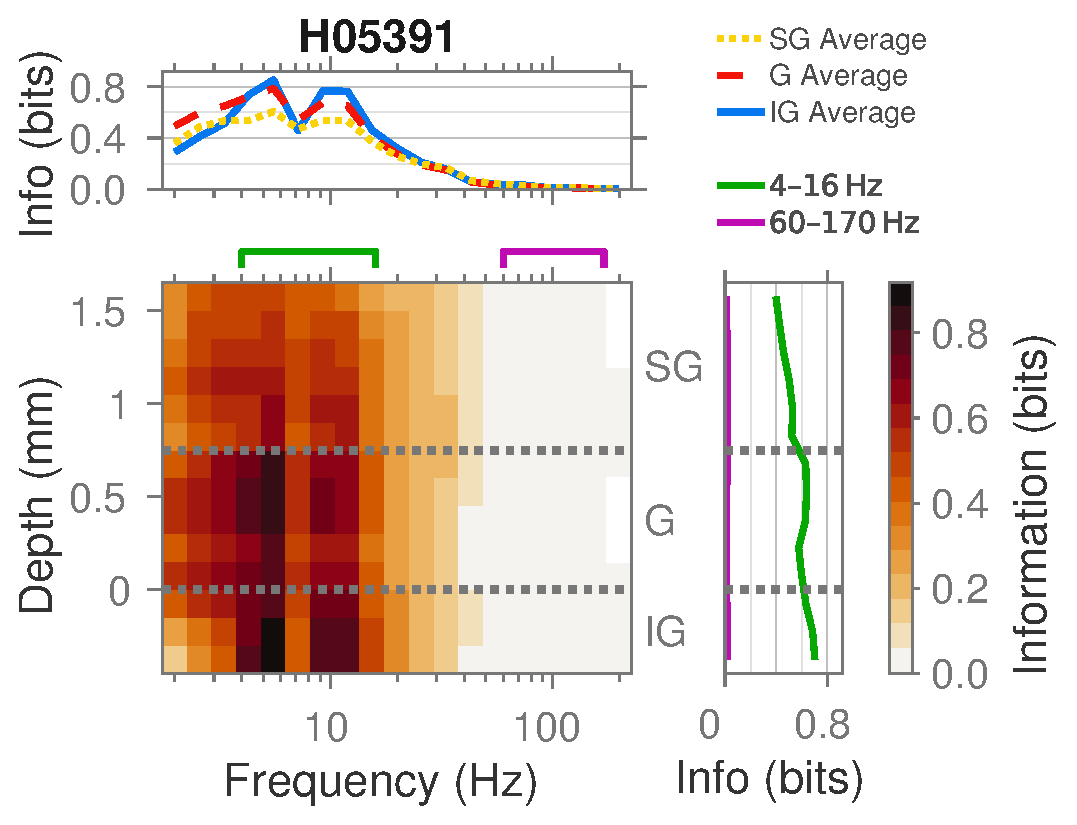
\includegraphics[scale=.4]{phaseinfo/fig3set-info-Cln-phase-H05391-compzonescb-legend.eps}
% }
%     \hspace*{\fill}\hspace{.2cm}\hspace*{\fill}
%     \subfloat[\sesname{H05nm9}\label{fig:lam_phase_info_lfp_H05nm9}]{
%         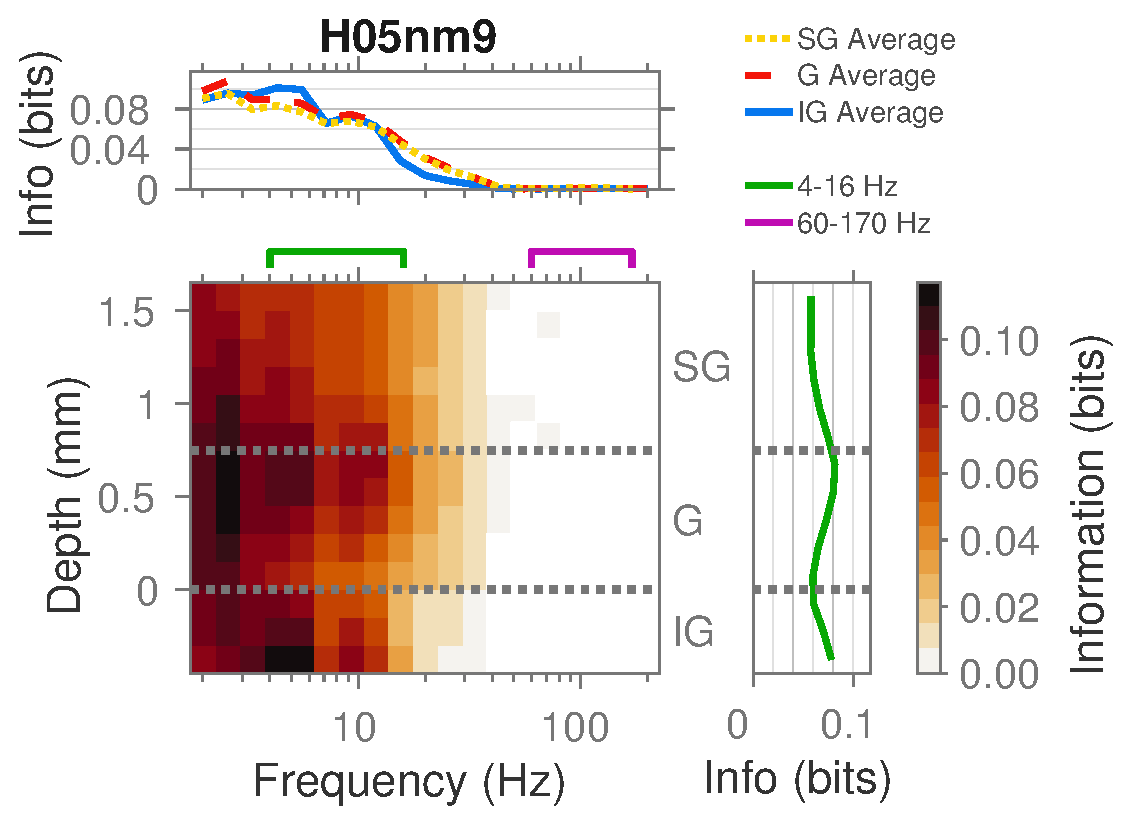
\includegraphics[scale=.4]{phaseinfo/fig3set-info-Cln-phase-H05nm9-compzonescb-legend.eps}
% }
%     \hspace*{\fill}
%     \\
%     \hspace*{\fill}
%     \subfloat[\sesname{H05nm7}\label{fig:lam_phase_info_lfp_H05nm7}]{
%         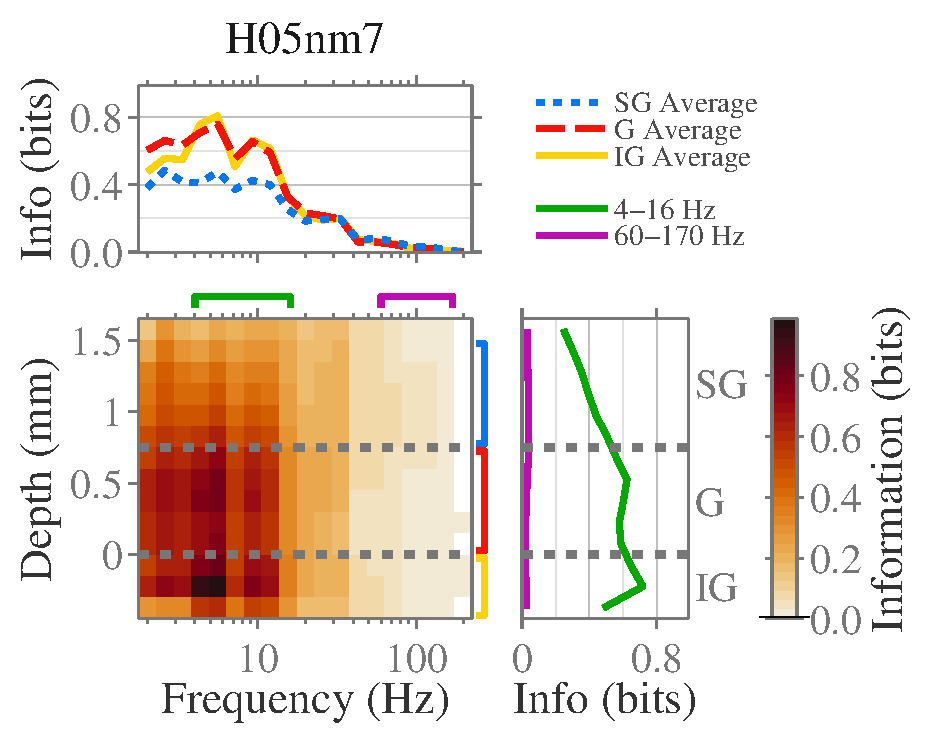
\includegraphics[scale=.4]{phaseinfo/fig3set-info-Cln-phase-H05nm7-compzonescb-legend.eps}
% }
%     \hspace*{\fill}\hspace{.2cm}\hspace*{\fill}
%     \subfloat[\sesname{E07nm1}\label{fig:lam_phase_info_lfp_E07nm1}]{
%         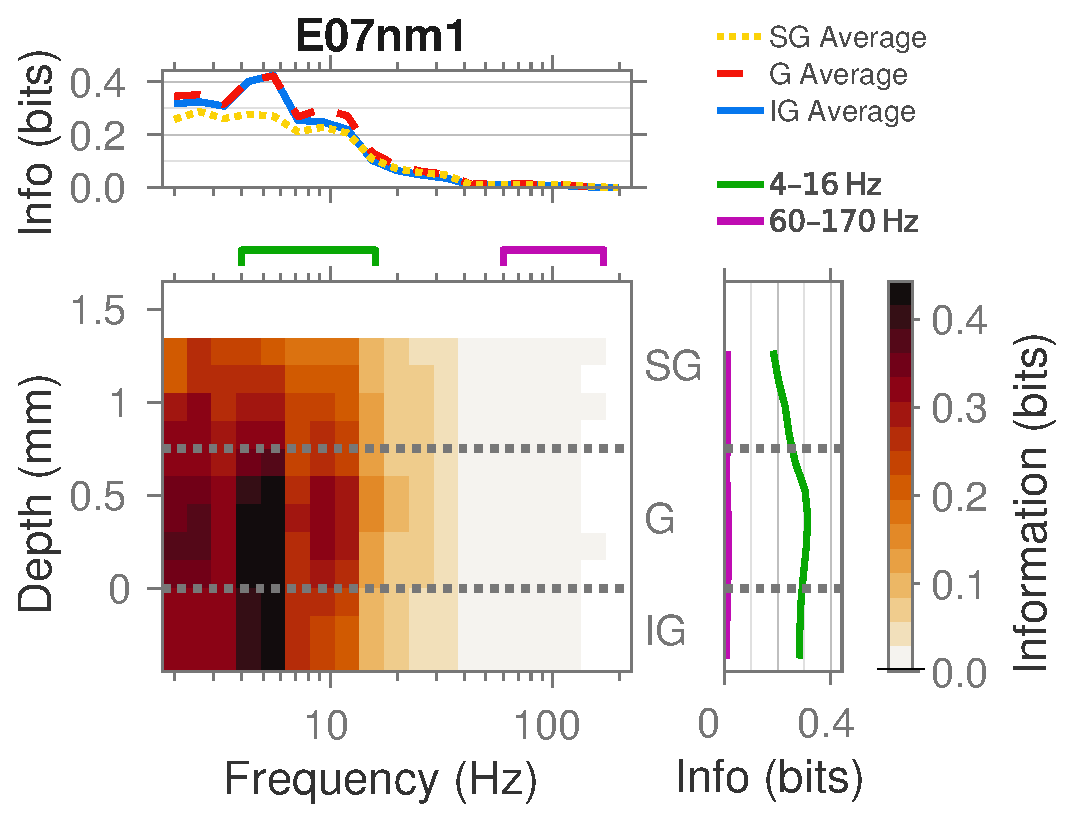
\includegraphics[scale=.4]{phaseinfo/fig3set-info-Cln-phase-E07nm1-compzonescb-legend.eps}
% }
%     \hspace*{\fill}
%     \\
%     \hspace*{\fill}
%     \subfloat[\sesname{F10nm1}\label{fig:lam_phase_info_lfp_F10nm1}]{
%         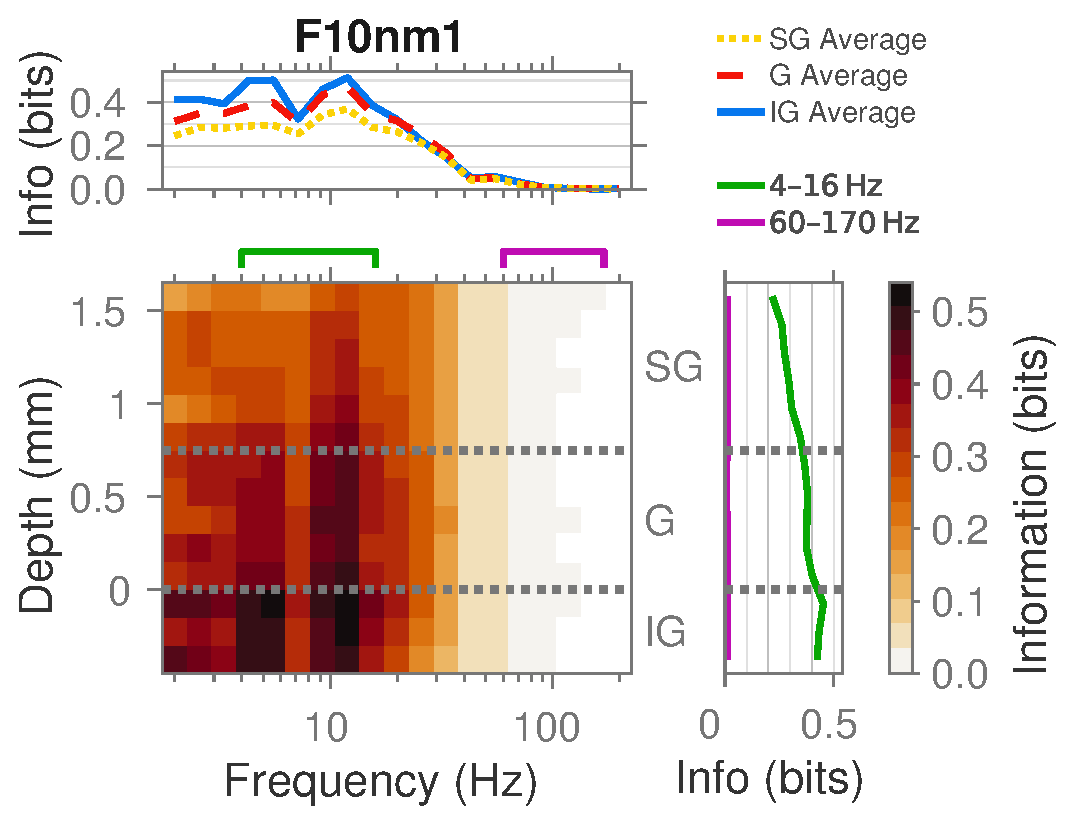
\includegraphics[scale=.4]{phaseinfo/fig3set-info-Cln-phase-F10nm1-compzonescb-legend.eps}
% }
%     \hspace*{\fill}\hspace{.2cm}\hspace*{\fill}
%     \subfloat[\sesname{J10nm1}\label{fig:lam_phase_info_lfp_J10nm1}]{
%         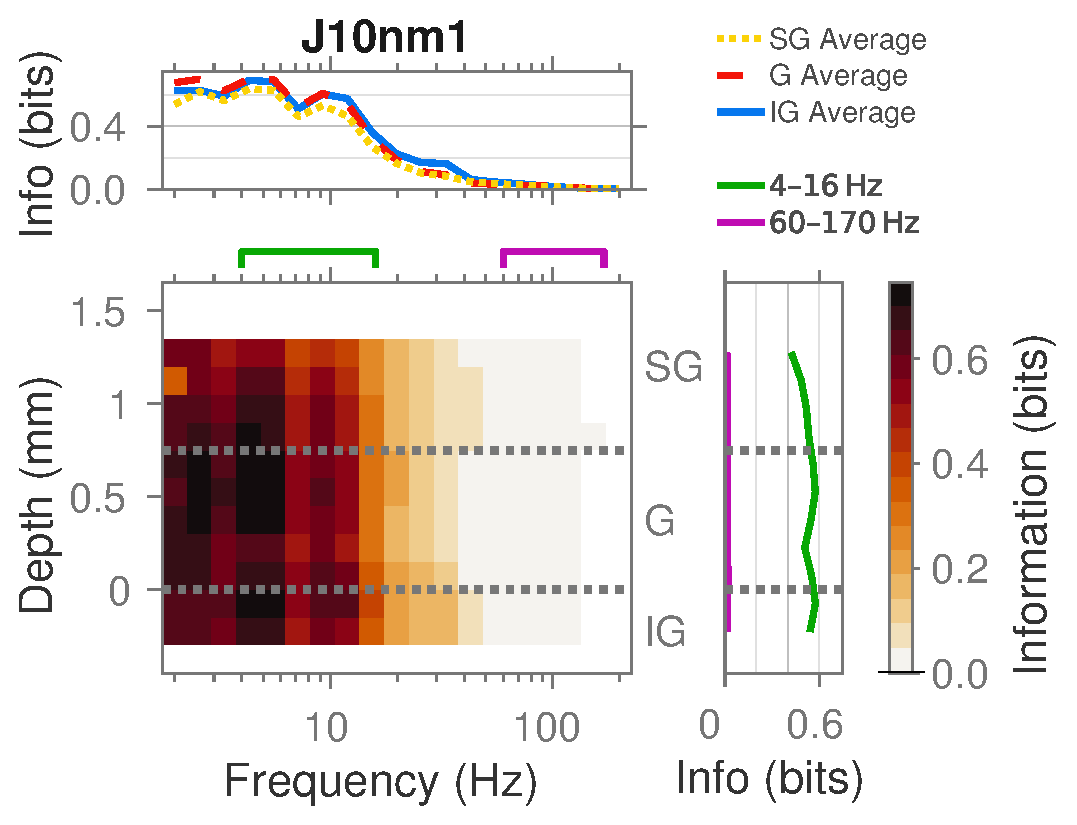
\includegraphics[scale=.4]{phaseinfo/fig3set-info-Cln-phase-J10nm1-compzonescb-legend.eps}
% }
%     \hspace*{\fill}
%     \caption{
% Information about the stimulus contained in the phase of the \ac{LFP}, as a function of frequency, by session.
% }
% \label{fig:lam_phase_info_lfp_sessions}
% \end{figure}


% \begin{figure}[htbp]
%     \centering
%     \hspace*{\fill}
%     \subfloat[\sesname{H05391}\label{fig:lam_phase_info_csd_H05391}]{
%         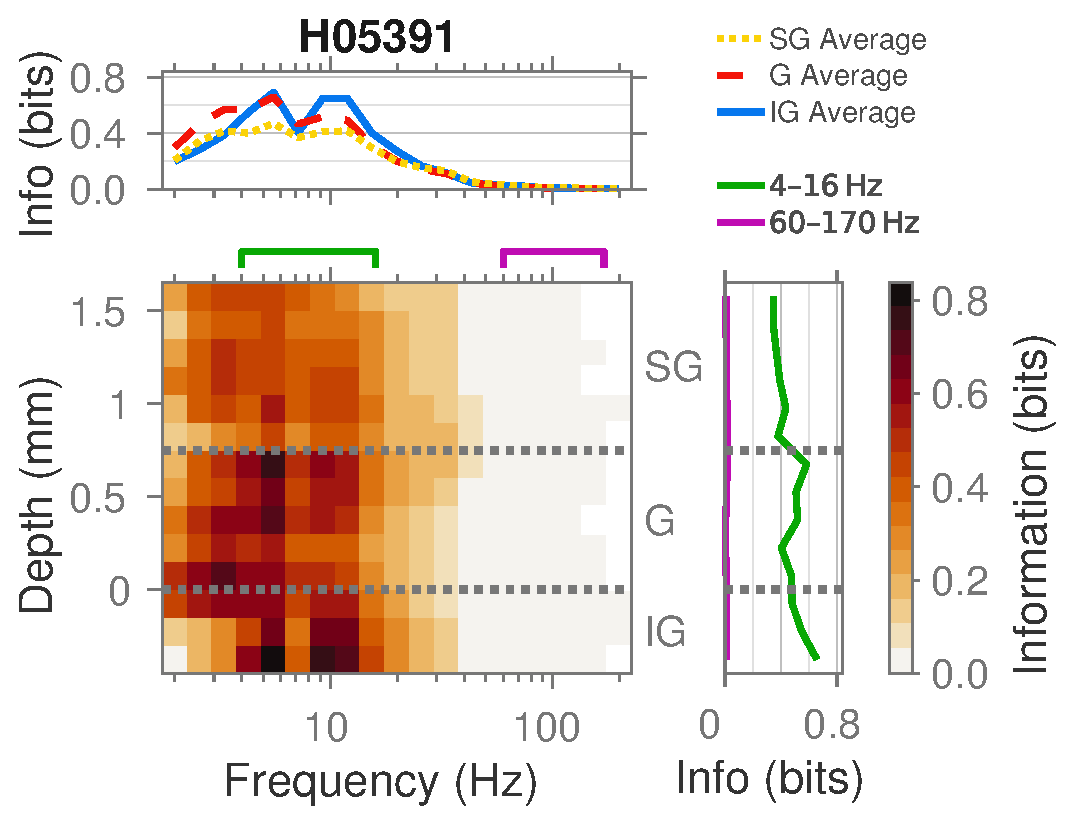
\includegraphics[scale=.4]{phaseinfo/fig3set-info-Csd-phase-H05391-compzonescb-legend.eps}
% }
%     \hspace*{\fill}\hspace{.2cm}\hspace*{\fill}
%     \subfloat[\sesname{H05nm9}\label{fig:lam_phase_info_csd_H05nm9}]{
%         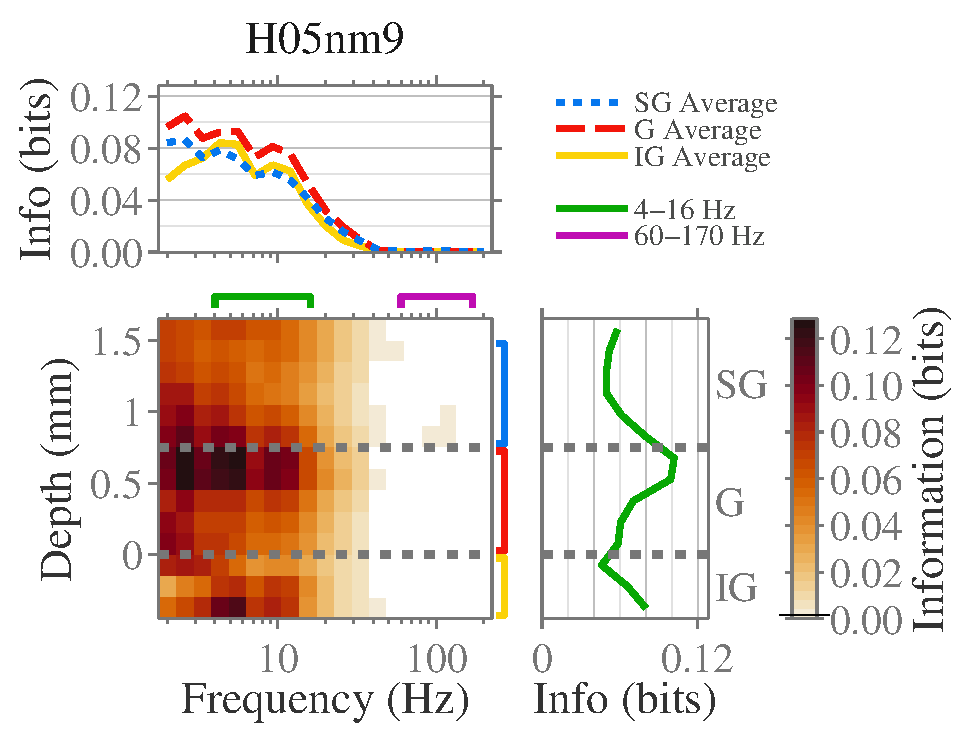
\includegraphics[scale=.4]{phaseinfo/fig3set-info-Csd-phase-H05nm9-compzonescb-legend.eps}
% }
%     \hspace*{\fill}
%     \\
%     \hspace*{\fill}
%     \subfloat[\sesname{H05nm7}\label{fig:lam_phase_info_csd_H05nm7}]{
%         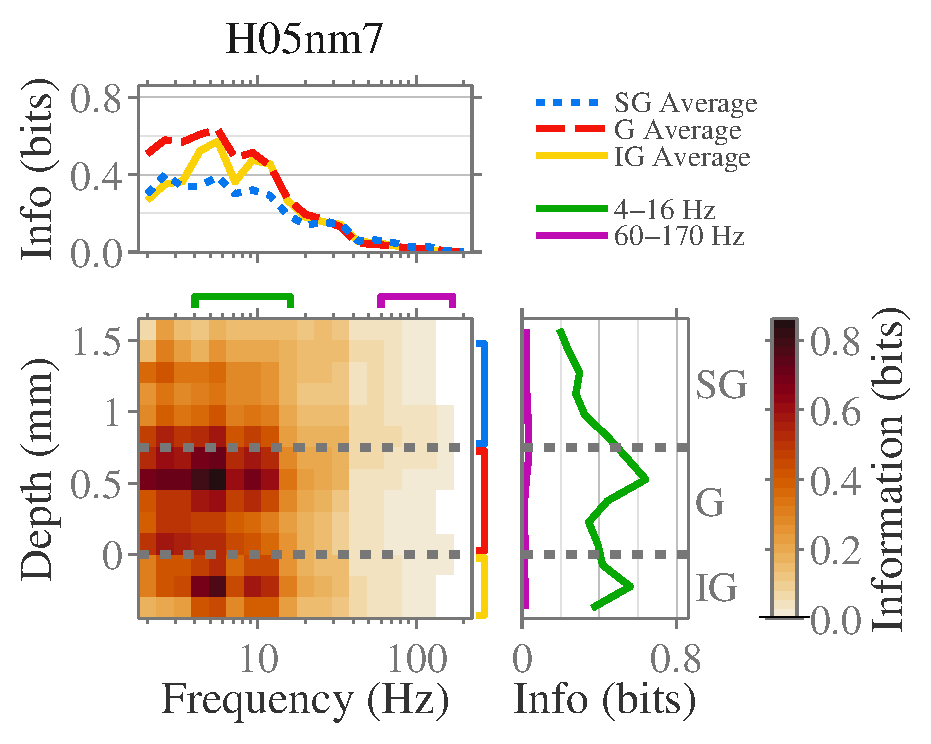
\includegraphics[scale=.4]{phaseinfo/fig3set-info-Csd-phase-H05nm7-compzonescb-legend.eps}
% }
%     \hspace*{\fill}\hspace{.2cm}\hspace*{\fill}
%     \subfloat[\sesname{E07nm1}\label{fig:lam_phase_info_csd_E07nm1}]{
%         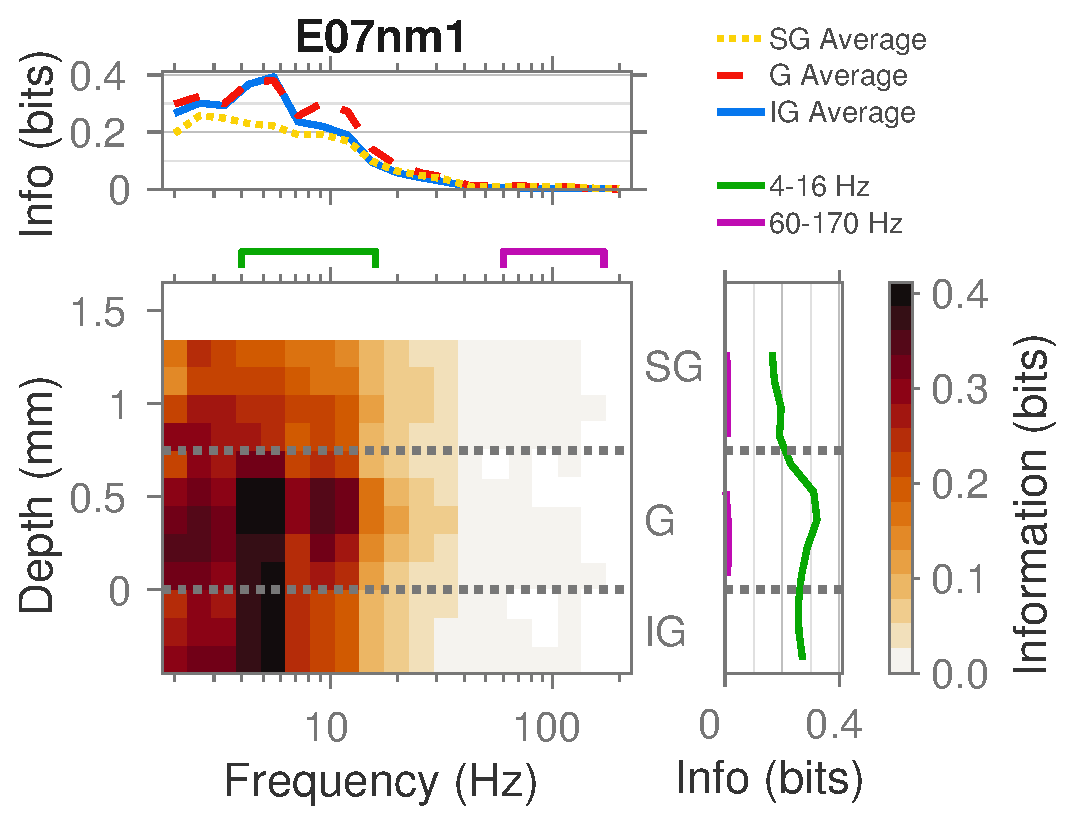
\includegraphics[scale=.4]{phaseinfo/fig3set-info-Csd-phase-E07nm1-compzonescb-legend.eps}
% }
%     \hspace*{\fill}
%     \\
%     \hspace*{\fill}
%     \subfloat[\sesname{F10nm1}\label{fig:lam_phase_info_csd_F10nm1}]{
%         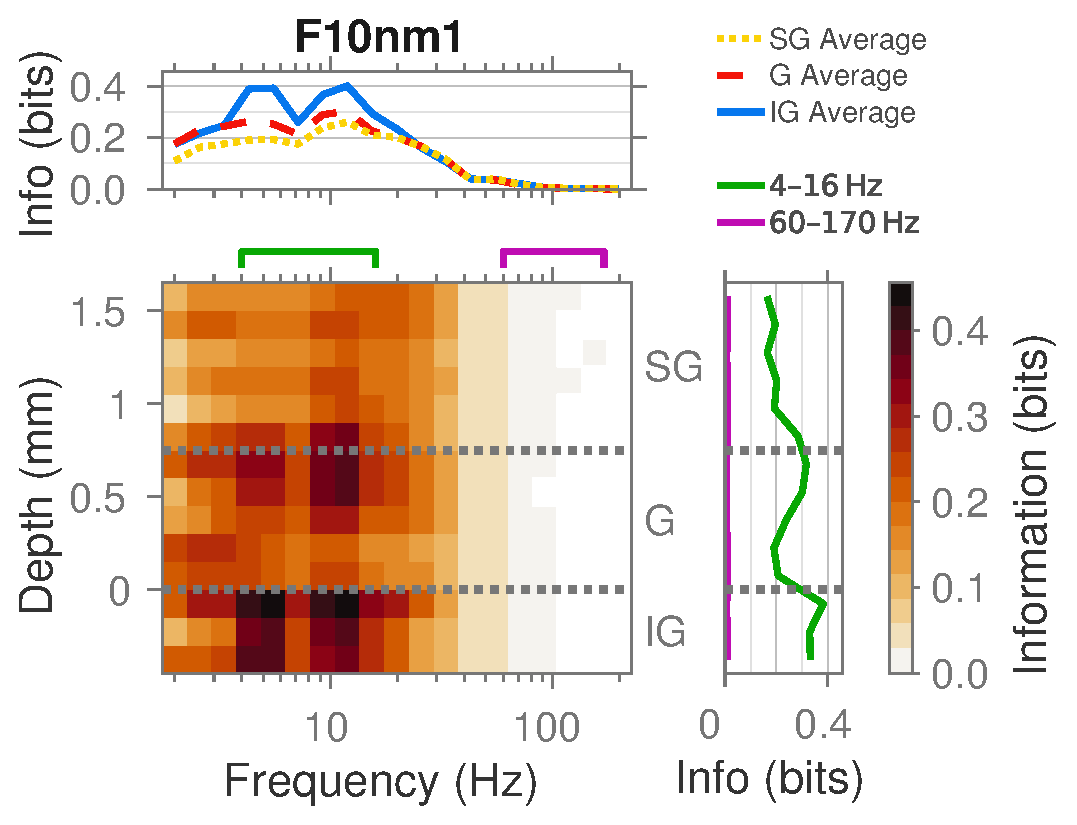
\includegraphics[scale=.4]{phaseinfo/fig3set-info-Csd-phase-F10nm1-compzonescb-legend.eps}
% }
%     \hspace*{\fill}\hspace{.2cm}\hspace*{\fill}
%     \subfloat[\sesname{J10nm1}\label{fig:lam_phase_info_csd_J10nm1}]{
%         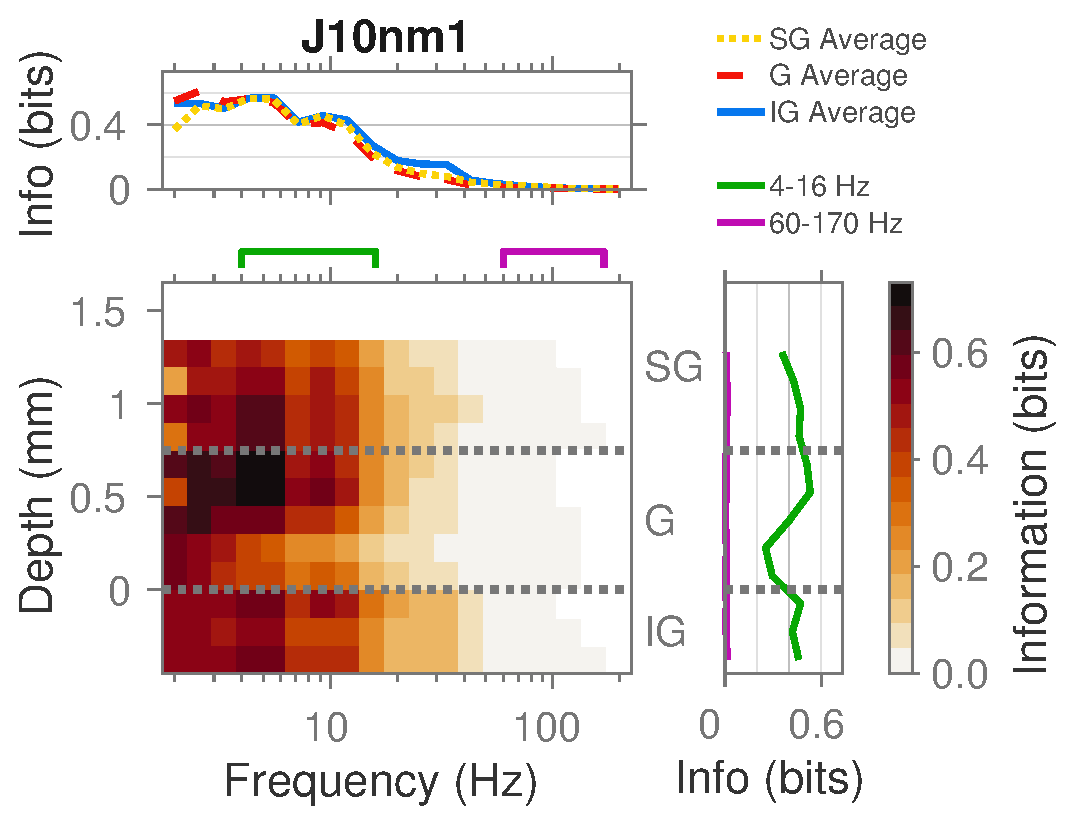
\includegraphics[scale=.4]{phaseinfo/fig3set-info-Csd-phase-J10nm1-compzonescb-legend.eps}
% }
%     \hspace*{\fill}
%     \caption{
% Information about the stimulus contained in the phase of the \ac{CSD}, as a function of frequency, by session.
% }
% \label{fig:lam_phase_info_csd_sessions}
% \end{figure}

%-------------------------------------------------------------------------------
\subsection{Phase-phase redundancy}
%-------------------------------------------------------------------------------

These results prompt us to consider the redundancy of the phase of oscillations.
Do the phases of oscillations at different frequencies convey information about the same aspects of the stimulus, as we found for the information in the power of the same oscillations?
Furthermore, how is the information in the phase related to the information in the power?

First, we consider the relationship between the phases of the frequency bands ($50\%$ bandwidth) occurring at the same cortical depths as one another.
As shown in \autoref{fig:lam_phase_cxfrq_info}, we find that pairs of frequency bands \SI{<40}{Hz} contain synergistic information about the stimulus, except for overlapping frequency bands which show redundancy.
This means that knowing the phase of two such frequency bands provides more information about the stimulus than the information in the two of them individually.
The observed synergy is similar across all pairs of frequencies \SI{<40}{Hz}, which suggests the cause is intrinsic to the Fourier transform its phase in general, and not specific to the cortical oscillation data we are considering.
In particular, peaks and troughs in the overall \ac{CSD} signal occur when multiple frequency components reach $0$ and $\pi$ radians, respectively.
As we already demonstrated in \autoref{sec:lam_scnchg} for the information in the power (and will demonstrate for the phase in \autoref{sec:lam_phase_scnchg}), scene transitions provide an important stimulation drive for low frequency oscillations.
In particular, scene cuts induce similar oscillation waveforms on each of their occurrences (not shown, but similar to the stimulus-onset stereotyped response shown in \autoref{fig:lam_align_csd}).
Since the distribution over phase for any single frequency component is uniform, coincident phases for a pair of frequencies are much more informative about peaks and troughs in the signal.
%
% The phase of the signal is constrained to the range $[0,2\pi)$ and we measure a value in this range for every frame of the movie stimulus.
% Even if there is little or no oscillation in that frequency at a measurement time, we always record a phase from within this range.
% Consequently, it may be that most measurements of the phase occur at times which are uninformative
%
% Intuitively, it seems likely that this situation arises from the properties of the Fourier transform and the power distribution of the stimulus.
% The power of the \ac{LFP} and \ac{CSD} vary smoothly with over the frequency domain, with an approximately $\nicefrac{1}{f}$, or power law, relationship (\autoref{fig:lam_info}).
% There is a known phenomenon which occurs for natural images: the power spectral density varies smoothly with a power law and so the phase of the Fourier transformation alone encodes the structural information in the image (\citealp[Chapter~3, page~62]{Jahne1991}; \citealp[Chapter~5, page~121]{Hyvarinen2009}).
% Using the Fourier transformation, we decompose the raw \ac{CSD} into a collection of sinusoidal waves at different frequencies
% Irrespective of which pair of frequency bands we consider,
%

For frequencies above \SI{40}{Hz}, the redundancy of the phase with other frequency bands was not significant, due to the low amount of information this frequency range.

\begin{figure}[htbp]
\centering
\hspace*{\fill}
\subfloat[Redundancy.\label{fig:lam_phase_cxfrq_info_red}]{
    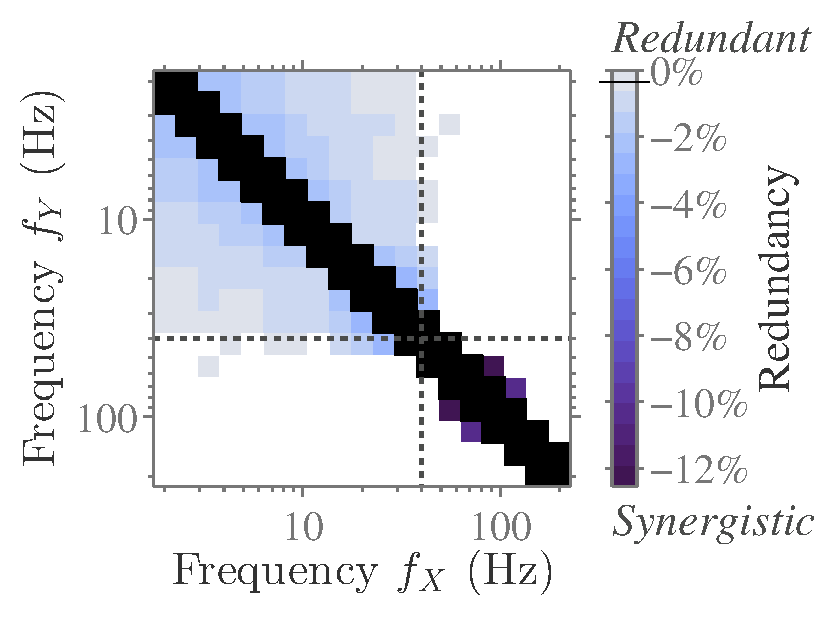
\includegraphics[scale=.5]{%
redundancy-cxsfrq/cxsfrq-pcred_phase-phase_avg-log_nodiag.eps}}
\hspace*{\fill}\hspace{.2cm}\hspace*{\fill}
\subfloat[Information gain.\label{fig:lam_phase_cxfrq_info_gain}]{
    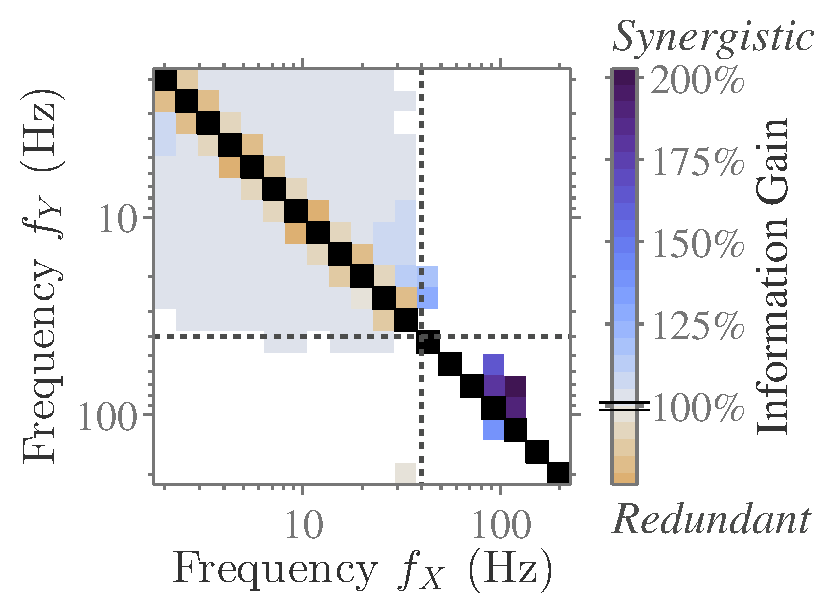
\includegraphics[scale=.5]{%
redundancy-cxsfrq/cxsfrq-pcgain-i2d2_phase-phase_avg-log_nodiag.eps}}
\hspace*{\fill}
    \caption{
\captionemph{Information redundancy between the phase of \ac{CSD} frequency components.}
\protect\subref{fig:lam_phase_cxfrq_info_red}:~Redundancy (as defined in \autoref{eq:redundancy}) between pairs of frequencies, averaged over all cortical recording depths, then averaged over \num{6} sessions.
Each datapoint was tested for statistical significance using bootstrapping, and non-significant values are shown in white (the median threshold for statistical significance is shown as a line across the colour bar).
The leading diagonal, which is trivially redundant, is removed (black).
\protect\subref{fig:lam_phase_cxfrq_info_gain}:~Same as \protect\subref{fig:lam_cxfrq_red}, but for the asymmetric information gain $\operatorname{InfoGain}\left(Y\to\left\{X,Y\right\};S\right)$ (defined in \autoref{eq:infogain}).
}
\label{fig:lam_phase_cxfrq_info}
\end{figure}


We also computed the signal and noise correlation, using the methodology described in \autoref{sec:pl_phase_correlation}.
Beyond the trivially positively correlated signal correlation of neighbouring frequency bands, as shown in \autoref{fig:lam_signal_corr_phase} we find there are some pairs of frequencies which are positively correlated (phase of \SI{10}{Hz} and \SI{30}{Hz}) and negatively correlated (phase of \SI{3}{Hz} and \SI{30}{Hz}).
The level of signal correlation is lower than we observed for the power-power correlation across frequency (see \autoref{fig:lam_cxfrq_cor}).
% though the two do measure different things
The noise correlation was small and positive for all pairs of phases considered, shown in \autoref{fig:lam_noise_corr_phase}.


\begin{figure}[htbp]
    \centering
    \hspace*{\fill}
    \subfloat[Signal correlation\label{fig:lam_signal_corr_phase}]{
        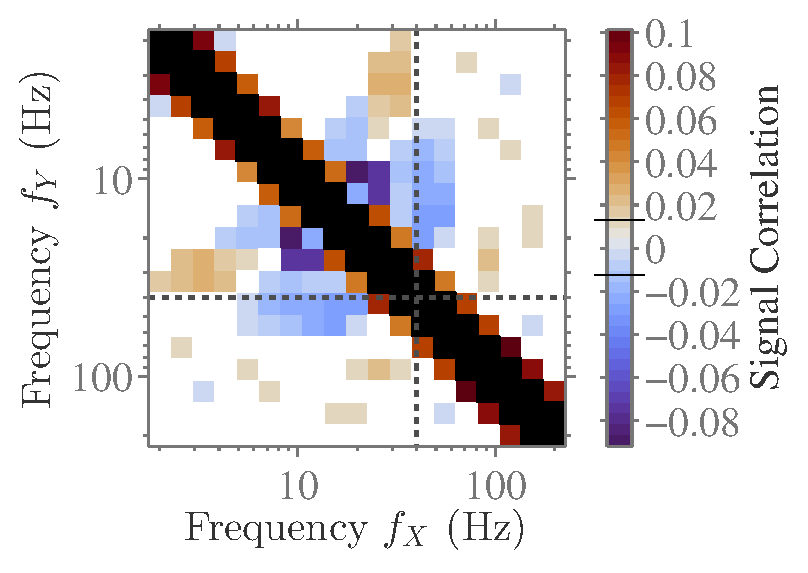
\includegraphics[scale=.5]{noisesigcorr/cxsfrq-signal-phase-phase-avg-log_nodiag.eps}
}
    \hspace*{\fill}\hspace{.2cm}\hspace*{\fill}
    \subfloat[Noise correlation\label{fig:lam_noise_corr_phase}]{
        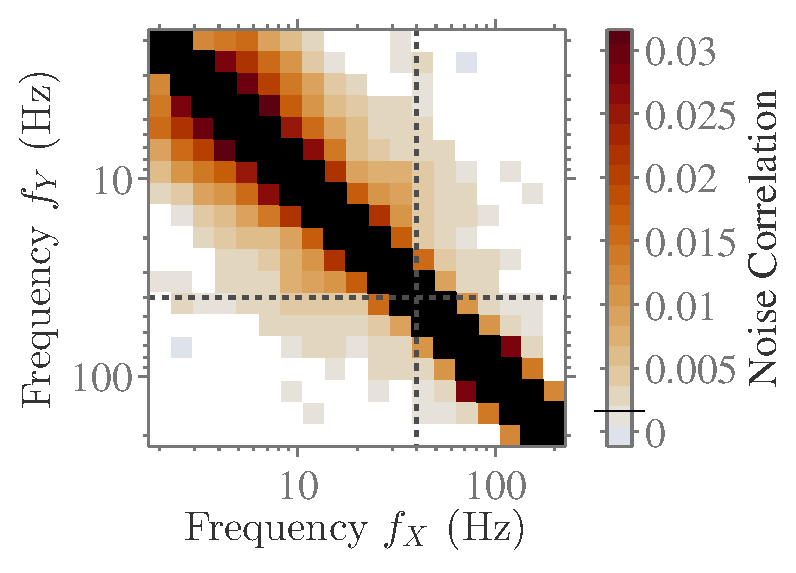
\includegraphics[scale=.5]{noisesigcorr/cxsfrq-noise-phase-phase-avg-log_nodiag.eps}
}
    \hspace*{\fill}
    \caption{
\captionemph{Correlation between phase of different \ac{CSD} frequency components.}
\protect\subref{fig:lam_signal_corr_phase}:~Signal correlation between the phase in pairs of frequencies, median across \numrange{12}{14} cortical recording sites, mean across \num{6} sessions.
The leading diagonal, which is trivially perfectly correlated, and second diagonal, which is highly correlated due to the $50\%$ overlap between neighbouring frequency bands, are removed (black).
\protect\subref{fig:lam_noise_corr_phase}:~Noise correlation between the phase in pairs of frequencies, median across \numrange{12}{14} cortical recording sites, mean across \num{6} sessions.
Non-significant datapoints are shown in white, with minimum and maximum significance thresholds indicated by the black lines across the colour bar.
}
\label{fig:lam_noisesignal_corr_phase}
\end{figure}


Unlike when we considered the information in the cortical power, neither the redundancy between phases of frequencies, nor signal and noise correlation structure, provided us with sufficient motivation to chose any particular frequency bands to isolate.
Therefore, we continue to examine the \SIrange{4}{16}{Hz} and \SIrange{60}{170}{Hz} frequency bands which we arrived at from our analysis of the information encoded in cortical power.
This allows us to compare the information in the phase and power of the same bands.


%-------------------------------------------------------------------------------
\subsection{Phase-power redundancy}

Similar to the above, we can also consider the redundancy between information in the power and phase as a function of their frequencies.
As shown in \autoref{fig:lam_cxfrq_powerphase_info}, we find that some pairs of power and phase have redundant information about the stimulus, some synergistic, and others approximately independent.


\begin{figure}[htbp]
    \centering
    \subfloat[Redundancy.\label{fig:lam_cxfrq_powerphase_info_red}]{
        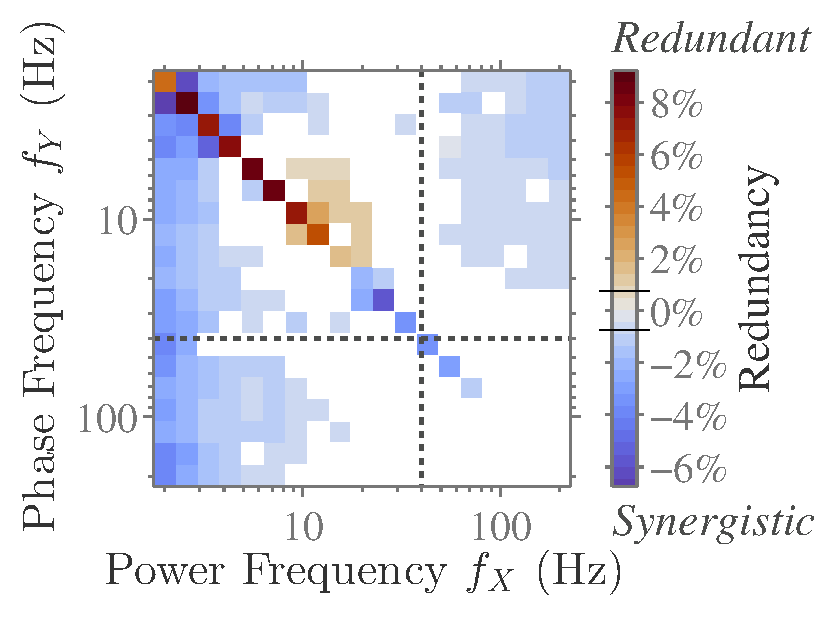
\includegraphics[scale=.5]{redundancy-cxsfrq/cxsfrq-pcred_phase-power_avg-log_nodiag.eps}
}
    \\
    \hspace*{\fill}
    \subfloat[$\operatorname{InfoGain}\left(\text{Phase}\to\left\{\text{Phase},\text{Power}\right\};S\right)$.\label{fig:lam_cxfrq_phasepower_gain}]{
        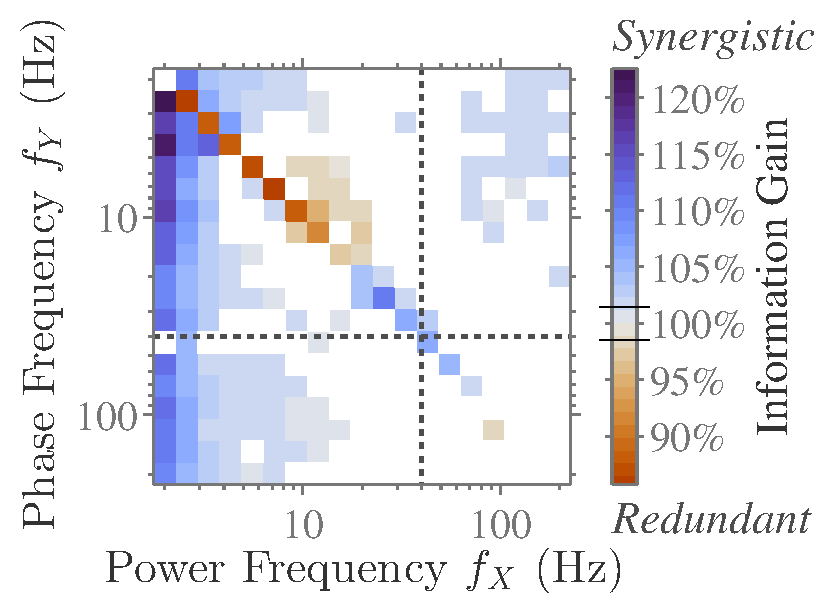
\includegraphics[scale=.5]{redundancy-cxsfrq/cxsfrq-pcgain-i2d2_phase-power_avg-log_nodiag.eps}
}
    \hspace*{\fill}\hspace{.2cm}\hspace*{\fill}
    \subfloat[$\operatorname{InfoGain}\left(\text{Power}\to\left\{\text{Phase},\text{Power}\right\};S\right)$.\label{fig:lam_cxfrq_powerphase_gain}]{
        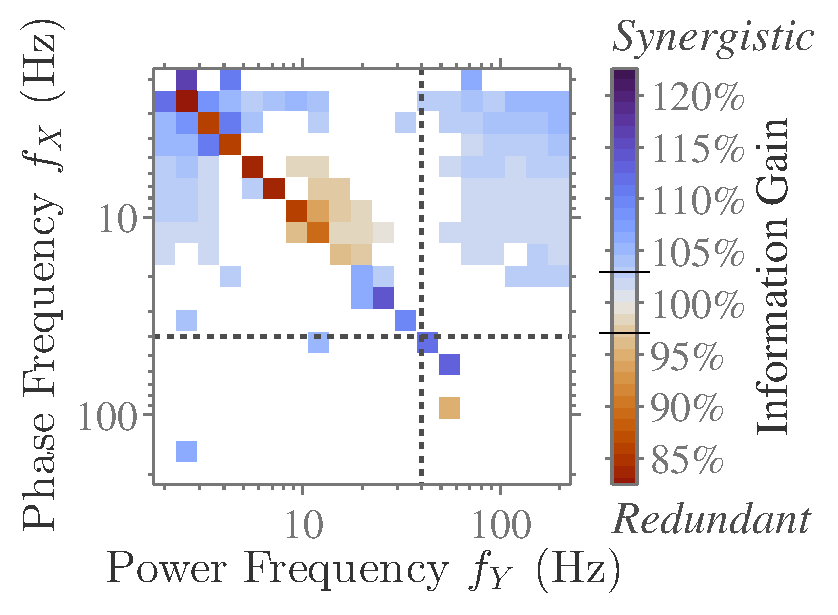
\includegraphics[scale=.5]{redundancy-cxsfrq/cxsfrq-pcgain-i2d2_power-phase_avg-log_nodiag_flipped.eps}
}
    \hspace*{\fill}
    \caption{
\captionemph{Information redundancy between the phase and power of \ac{CSD} frequency components.}
\protect\subref{fig:lam_cxfrq_powerphase_info_red}:~Redundancy (as defined in \autoref{eq:redundancy}) between phase and power, averaged over all cortical recording depths, then averaged over \num{6} sessions.
Each datapoint was tested for statistical significance using bootstrapping, and non-significant values are shown in white (the median threshold for statistical significance is shown as a line across the colour bar).
\protect\subref{fig:lam_cxfrq_phasepower_gain}:~Same as \protect\subref{fig:lam_cxfrq_powerphase_info_red}, but for the asymmetric information gain when Phase is already known and Power is revealed (see \autoref{eq:infogain}).
\protect\subref{fig:lam_cxfrq_powerphase_gain}:~Same as \protect\subref{fig:lam_cxfrq_phasepower_gain}, but for the information gain when Power is already known and Phase is revealed.
}
\label{fig:lam_cxfrq_powerphase_info}
\end{figure}

There is significant redundancy between \SIrange{5}{15}{Hz} phase \SIrange{10}{20}{Hz} power, though the effect size is small.
Synergy is found between the phase (across all frequencies) and the power of oscillations below \SI{10}{Hz}, with a notable gain relative to the amount of information the power of these frequencies (see \autoref{fig:lam_cxfrq_phasepower_gain}).
We also see synergy between the phase of frequencies below \SI{20}{Hz} with the power in higher frequencies (\SI{>60}{Hz}).
These findings could be caused by a coupling of the envelope amplitude of the power for oscillations in one frequency band with the phase of oscillations in another band, which we consider in \autoref{sec:lam_cfc}.

% \begin{figure}[htbp]
%     \centering
%     \hspace*{\fill}
%     \subfloat[Signal correlation\label{fig:lam_signal_corr_phase_power}]{
%         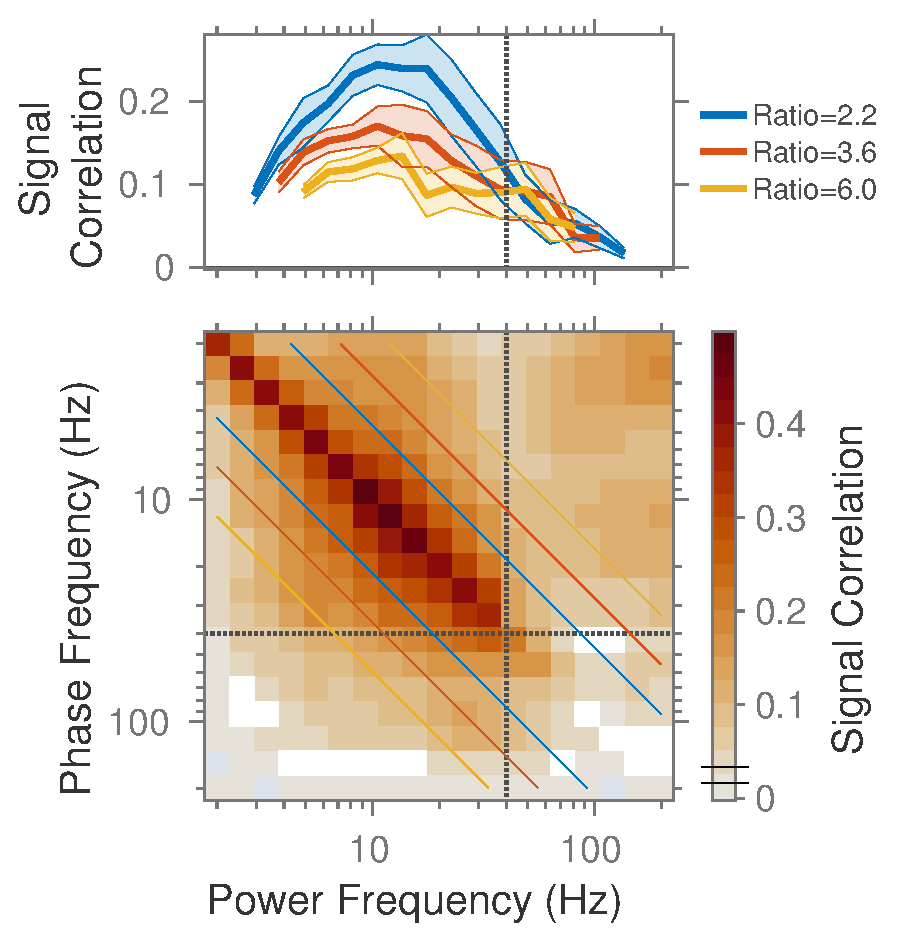
\includegraphics[scale=.45]{noisesigcorr/cxsfrq-signal-phase-power-avg-log.eps}
% }
%     \hspace*{\fill}\hspace{.2cm}\hspace*{\fill}
%     \subfloat[Noise correlation\label{fig:lam_noise_corr_phase_power}]{
%         %\includegraphics[scale=.45]{noisesigcorr/cxsfrq-noise-phase-power-avg-log.eps}
%         <code running>
% }
%     \hspace*{\fill}
%     \caption{Phase correlation with power
% \protect\subref{fig:lam_signal_corr_phase_power}:~Signal correlation.
% \protect\subref{fig:lam_noise_corr_phase_power}:~Noise correlation.
% }
% \label{fig:lam_noisesignal_corr_phase_power}
% \end{figure}


%-------------------------------------------------------------------------------
%\FloatBarrier
\subsection{Cross-channel, cross-depth redundancy}
%-------------------------------------------------------------------------------

Next, we consider how the information in the cortical phase is related to the information in the power and \ac{MUA} across the cortical depth.
We computed the redundancy between the \SIrange{4}{16}{Hz} phase and the \SIrange{4}{16}{Hz} power, \SIrange{60}{170}{Hz} power and \ac{MUA} (see figure \autoref{fig:lam_signal_red_depth}).

We found the \SIrange{4}{16}{Hz} phase at \ac{G} and \ac{SG} depths was redundant with the phase at other \ac{G} and \ac{SG} cortical depths, but mostly independent of the phase in \ac{IG}.
The phase in \ac{IG} is redundant to the phase at other \ac{IG} depths.
This suggests compartmentalisation of the \SIrange{4}{16}{Hz} frequency band, with two independent cortical oscillations occurring in this band but generated at (and localised in) two different cortical depths.
The results for signal (\autoref{fig:lam_signal_corr_depth}) and noise (\autoref{fig:lam_noise_corr_depth}) correlation support this view, as there is less correlation between \ac{G} or \ac{SG} phase and \ac{IG} phase than there is within either compartment.


\begin{figure}[htbp]
\centering
\subfloat[Redundancy.\label{fig:lam_signal_red_depth}]{
    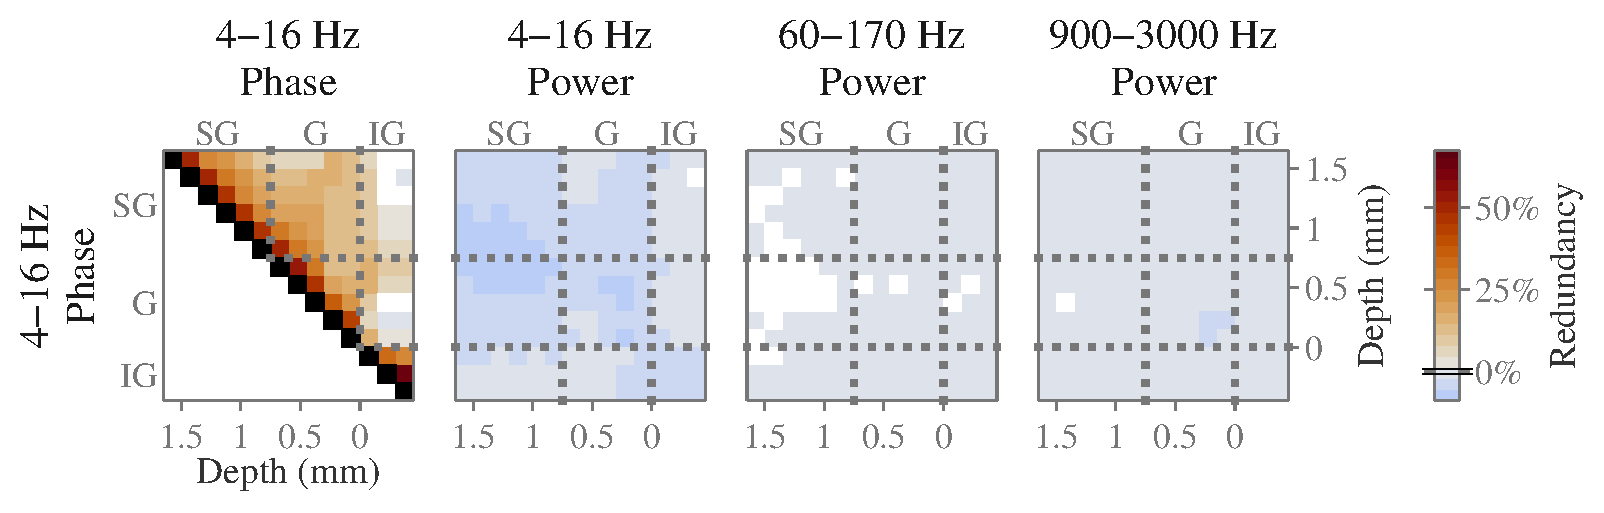
\includegraphics[scale=.5]{redundancy-cxschn/bndflt4-1-pcred-none-avg-lag=0s_paper.eps}
}
\\
\subfloat[Signal correlation.\label{fig:lam_signal_corr_depth}]{
    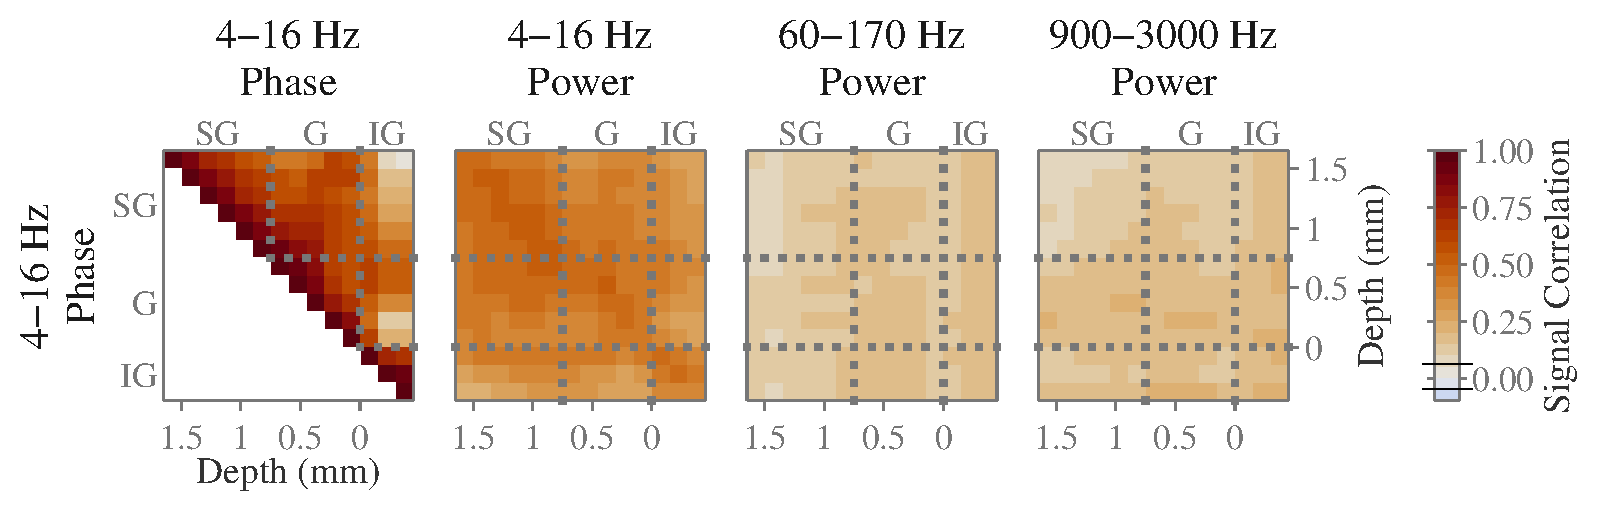
\includegraphics[scale=.5]{noisesigcorr/bndflt4-1-signal-avg_paper.eps}
}
\\
\subfloat[Noise correlation.\label{fig:lam_noise_corr_depth}]{
    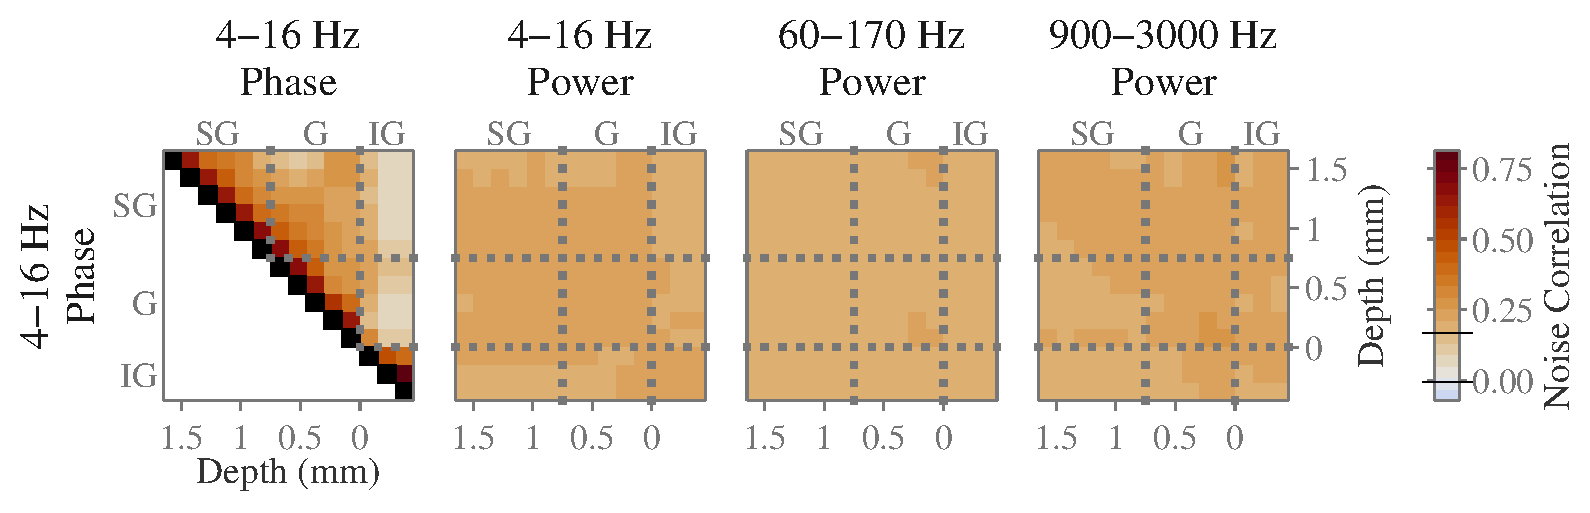
\includegraphics[scale=.5]{noisesigcorr/bndflt4-1-noise-avg_paper.eps}
}
\caption{
\captionemph{Redundancy of \SIrange{4}{16}{Hz} \ac{CSD} phase with \SIrange{4}{16}{Hz} power, \SIrange{60}{170}{Hz} power and \ac{MUA} (\SIrange{900}{3000}{Hz} power).}
\protect\subref{fig:lam_signal_red_depth}:~Redundancy (as defined in \autoref{eq:redundancy}) between phase and power.
Non-significant datapoints are shown in white, with median significance threshold (positive and negative) indicated by the black lines across the colour bar.
\protect\subref{fig:lam_signal_corr_depth}:~Signal correlation, reported as circular-circular correlation coefficient between phases and the circular-linear correlation coefficient between phase and power (see \autoref{sec:pl_phase_correlation}).
Non-significant datapoints are shown in white, with minimum and maximum significance thresholds indicated by the black lines across the colour bar.
\protect\subref{fig:lam_noise_corr_depth}:~Same as \protect\subref{fig:lam_signal_corr_depth}, but for noise correlation instead of signal correlation.
}
\label{fig:lam_noisesignal_corr_depth}
\end{figure}


The information about the stimulus in the \SIrange{4}{16}{Hz} phase was synergistic with the \SIrange{4}{16}{Hz} power.
Our explanation for this ties in with our explanation of the phase-phase synergy discussed above.
Since phase is uniformly instead of sparsely distributed, a secondary signal about the \ac{CSD} helps disambiguate whether the phase occurs during most, lower power, time points or during well-stereotyped waveform events or responses to the stimulus, which have higher power.
We note that the correlation with the \SIrange{4}{16}{Hz} phase is higher for the \SIrange{4}{16}{Hz} power than the higher frequency bands, whilst the noise is constant across all three, which supports this interpretation.

The information about the stimulus encoded in the \SIrange{4}{16}{Hz} phase appears to be different to the information encoded in the \SIrange{60}{170}{Hz} power and \ac{MUA} activity, which have balanced synergy and redundancy as shown in \autoref{fig:lam_signal_red_depth}.


%-------------------------------------------------------------------------------
\subsection{Information about scene cuts}
\label{sec:lam_phase_scnchg}
%-------------------------------------------------------------------------------

We computed the amount of information in the \ac{CSD} phase about scene transitions in the movie (agnostic about which of the scene transitions was occurring) in the same manner as described in \autoref{sec:lam_scnchg_method}.

In terms of number of bits encoded, the phase and power contain amount of information about the presence of scene cuts.
The fraction of information contained in the \ac{CSD} phase which is explained by scene transitions is smaller than we observed for the power (see \autoref{fig:lam_phs_scnchg}; \autoref{fig:lam_scnchg} for comparison).
This indicates that the phase encodes more properties of the stimulus than the power of cortical oscillations.


\begin{figure}[htbp]
\centering
% \hspace*{\fill}
% \subfloat[][As a function the duration after the scene cut horizon threshold.\label{fig:lam_phs_scnchg_dur}]{%
%     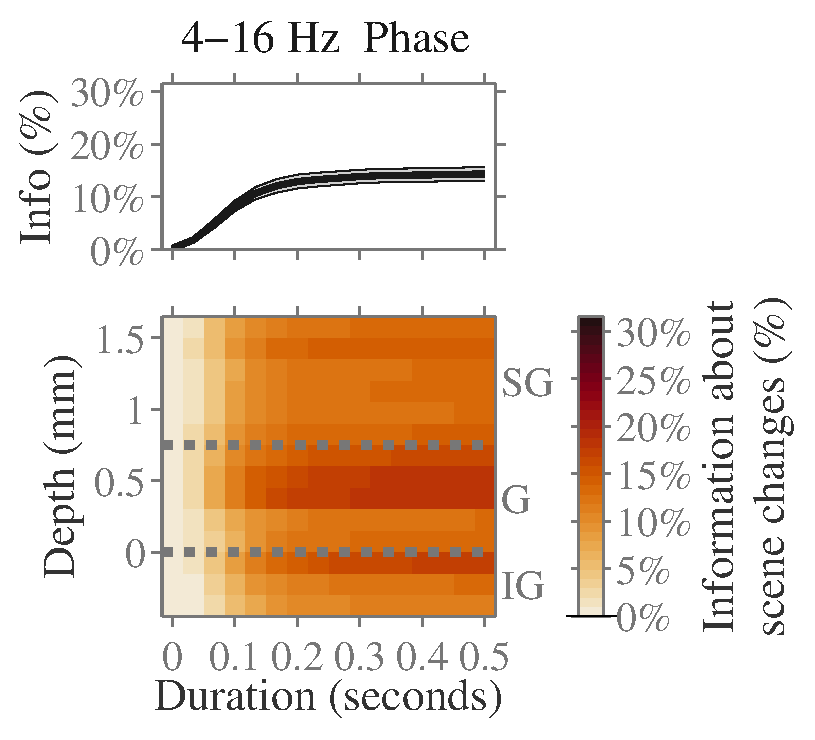
\includegraphics[scale=.5]{%
% scnchg/depth_v_scenecut-info_scnchg-dist_duration_avg_4-16Hz_phase.eps}}
% \hspace*{\fill}\hspace{.2cm}\hspace*{\fill}
% \subfloat[][Across a range of cortical frequencies.\label{fig:lam_phs_scnchg_frq}]{%
    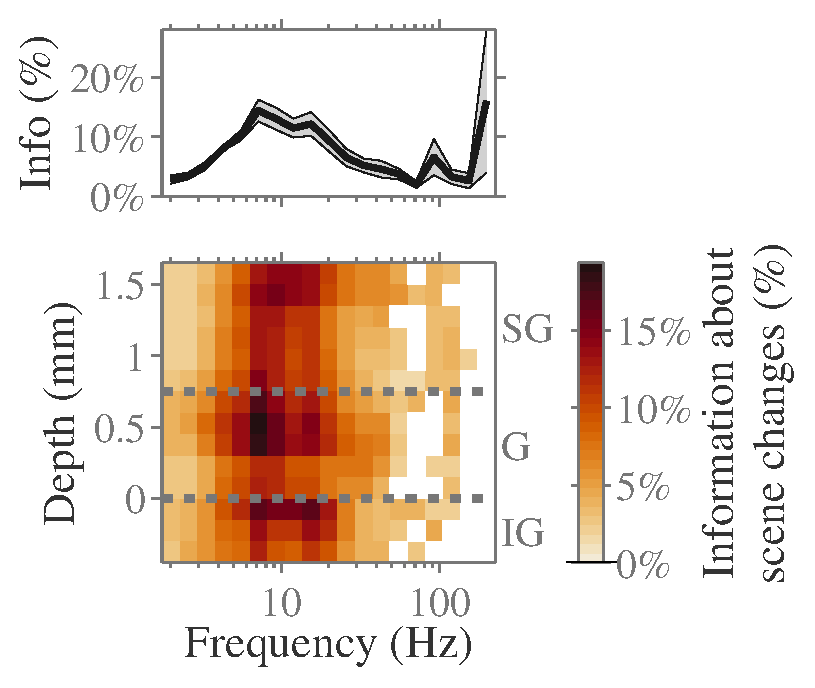
\includegraphics[scale=.5]{%
scnchg/frq-phase_v_depth_scenecut-info_scnchg-dist_0.200s_avg.eps}
% }
% \hspace*{\fill}
%
\caption{
\captionemph{Information about the presence of scene cuts.}
We computed the information about scene cuts as described in \autoref{sec:lam_scnchg_method}, and for each session expressed this as a proportion of the total information present before averaging across recording sessions.
% \protect\subref{fig:lam_phs_scnchg_dur}:~Information across the cortical depth for \SIrange{4}{16}{Hz} phase, averaged over \num{6} sessions.
Information values which were not significantly different from the bootstrap distribution are shown in white, with the median threshold for significance indicated by a black line across the colour bar.
Above, the average percentage of information explained by scene cuts over all cortical recording sites is shown, with the standard error across sessions indicated by the shaded region.
Information about scene cuts contained in a range of \ac{CSD} frequencies, in which we only considered the time since the last scene cut for the \SI{0.2}{\second} immediately following each.
}%
\label{fig:lam_phs_scnchg}
%
\end{figure}

In \autoref{sec:lam_scnchg}, we found that scene transitions explained more of the information in the cortical power for oscillations in the range \SIrange{7}{20}{Hz}.
For the phase of oscillations, the peak frequency range best explained by scene cuts is similar again, though the curve is flatter.


%-------------------------------------------------------------------------------
\subsection{Information about spatiotemporal components}
%-------------------------------------------------------------------------------

We computed the amount of information about changes in luminance at different spatiotemporal scales contained in the \ac{CSD} phase, the methodology for which is described in \autoref{sec:lam_tmf_method}.

The amount of information encoded in the \ac{CSD} phase is only around $10\%$ of the information encoded in the power (\autoref{fig:lam_phs_spatmf}; see \autoref{sec:lam_spatmf} for comparison).
This result is surprising, since we observed in \autoref{sec:lam_phase_scnchg} that the \ac{CSD} contains information a significant amount of information about scene cuts in the movie --- around \SI{0.06}{bits}, which is ten times more than we observe here.
These two results appear to be contradictory, since scene transitions typically involve sudden, coarse changes in the luminance of the stimulus.
But we note that the spatiotemporal distribution of information contained in the \SIrange{4}{16}{Hz} phase is the same as the distribution that for the \SIrange{4}{16}{Hz} power, though the distribution over depth is skewed towards deeper, \ac{IG}, cortical layers.


\begin{figure}[htbp]
\centering
    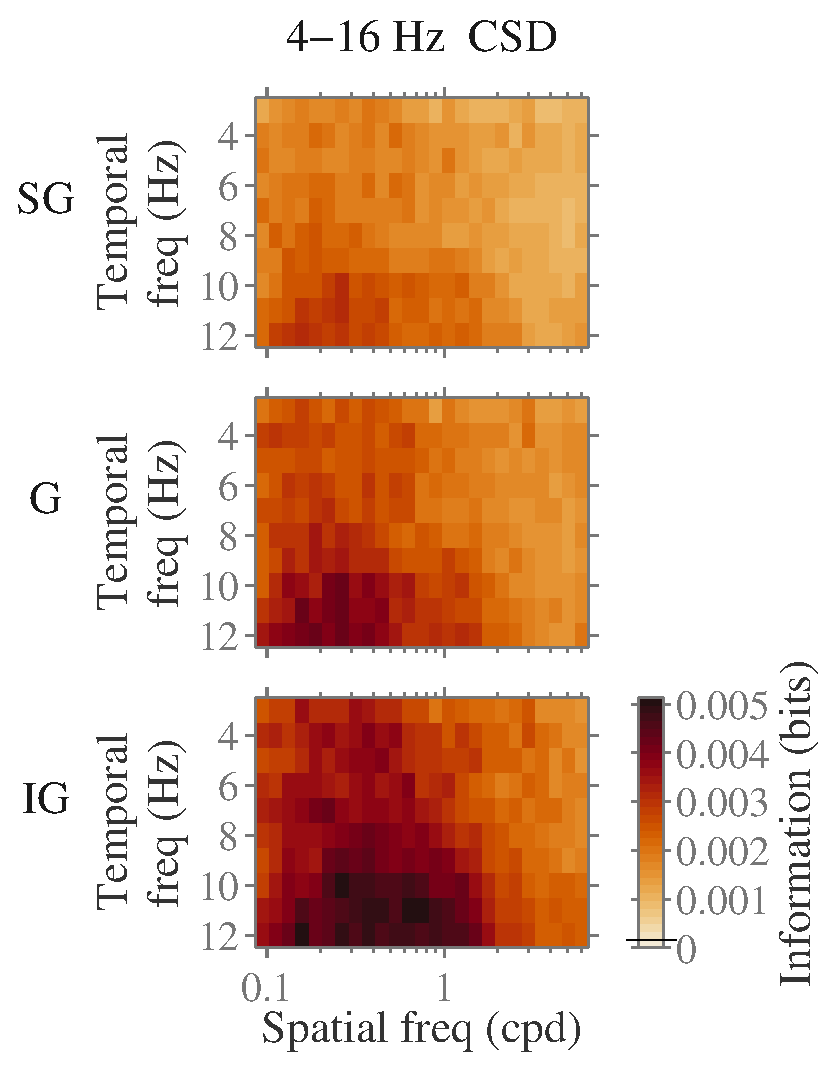
\includegraphics[scale=.5]{%
spatmf/tmf-v-spares-sggig-avg-spatmf2_4-16Hz_phase.eps}
\caption{%
\captionemph{Information contained in the \SIrange{4}{16}{Hz} \ac{CSD} phase about different spatiotemporal components.}
% Same as \autoref{fig:lam_spatmf}, but for phase.
The luminance of the movie was filtered in the spatial domain with using bandpass filters each with width one octave, and in the temporal domain with bandpass filters each with width \SI{6}{Hz}.
Datapoints are shown against the middle of the band on both $x$ and $y$.
Each row of panels corresponds to a different cortical depth, averaging over \ac{SG}, \ac{G} and \ac{IG} compartments, respectively.
Throughout all panels, the mean over \num{6} sessions is indicated.
Statistical significance thresholds were computed for each datapoint individually, and a typical significance threshold is shown by the black line across the colour bar.
}%
\label{fig:lam_phs_spatmf}
%
\end{figure}


How does this behaviour arise, when the \ac{CSD} power was observed to give similar results for both scene transitions and spatiotemporal changes?
Unlike the power, the phase changes is always changing rapidly --- it must change at a rate similar to the frequency of the filtered band --- whereas the envelope amplitude describing how the power changes over time can vary much more slowly.
Consequently, the power of the \ac{CSD} has a long autocorrelation duration and the phase does not.
This means that small perturbations in the differences between recorded and actual presentation times of the stimuli will not have much effect on the measured information in the power but will for the phase.
Consequently, the relationship between the spatiotemporal changes in the movie and the \ac{CSD} phase may not be well aligned across trials.


%-------------------------------------------------------------------------------
%\FloatBarrier
\subsection{Phase synchrony}
% \subsection{Phase synchrony, \SIrange{4}{16}{Hz}}
%-------------------------------------------------------------------------------

% \begin{figure}[htbp]
%     \centering
%     \hspace*{\fill}
%     \subfloat[Movie driven\label{fig:lam_phasestats_alpha_line_csd_movie}]{
%         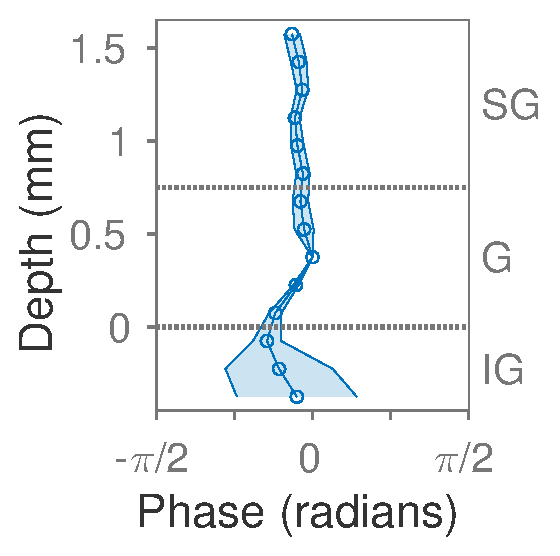
\includegraphics[scale=.45]{phasestats/movie1_Csd_phs4-16_dPhsTracebnd_5mean.eps}
% }
%     \hspace*{\fill}\hspace{.2cm}\hspace*{\fill}
%     \subfloat[Spontaneous\label{fig:lam_phasestats_alpha_line_csd_spont}]{
%         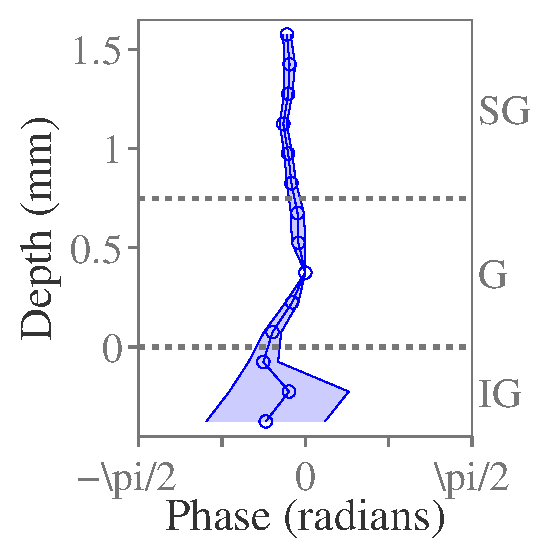
\includegraphics[scale=.45]{phasestats/spont_Csd_phs4-16_dPhsTracebnd_5mean.eps}
% }
%     \hspace*{\fill}
%     \caption{Phase correlation, \SIrange{4}{16}{Hz}.
% \protect\subref{fig:lam_phasestats_alpha_line_csd_movie}:~Movie driven.
% \protect\subref{fig:lam_phasestats_alpha_line_csd_spont}:~Spontaneous.
% }
% \label{fig:lam_phasestats_alpha_line_csd}
% \end{figure}

% \begin{figure}[htbp]
%     \centering
%     \hspace*{\fill}
%     \subfloat[Movie driven\label{fig:lam_phasestats_alpha_hist_csd_movie}]{
%         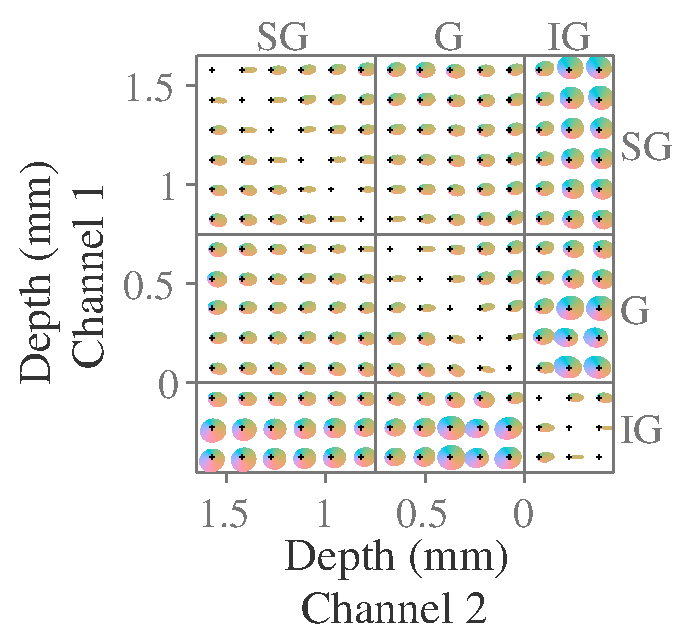
\includegraphics[scale=.45]{phasestats/movie1_Csd_phs4-16_dPhs_hist_5mean.eps}
% }
%     \hspace*{\fill}\hspace{.2cm}\hspace*{\fill}
%     \subfloat[Spontaneous\label{fig:lam_phasestats_alpha_hist_csd_spont}]{
%         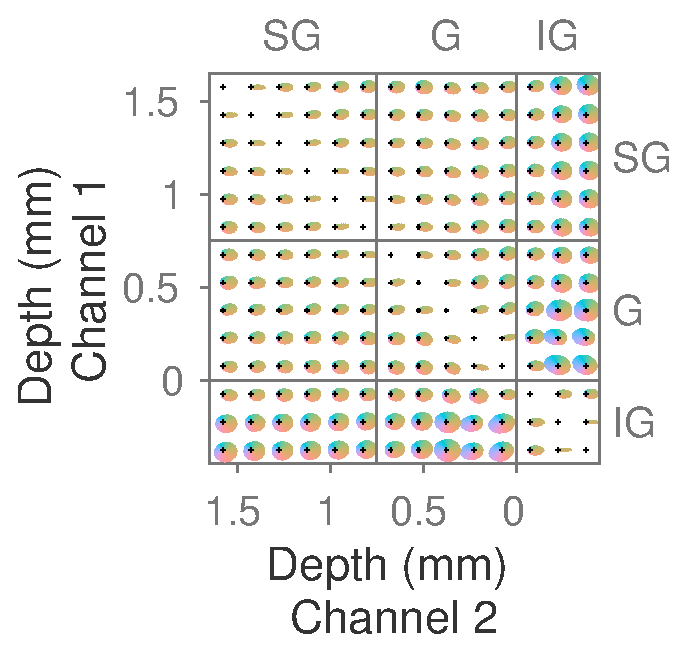
\includegraphics[scale=.45]{phasestats/spont_Csd_phs4-16_dPhs_hist_5mean.eps}
% }
%     \hspace*{\fill}
%     \caption{Phase correlation, \SIrange{4}{16}{Hz}.
% \protect\subref{fig:lam_phasestats_alpha_hist_csd_movie}:~Movie driven.
% \protect\subref{fig:lam_phasestats_alpha_hist_csd_spont}:~Spontaneous.
% }
% \label{fig:lam_phasestats_alpha_hist_csd}
% \end{figure}


We determined the average phase difference and the phase synchrony between oscillations in the \SIrange{4}{16}{Hz} across the cortical depth, for both stimulus driven and spontaneous activity.
As shown in \autoref{fig:lam_phasestats_alpha_combo_csd}, there is high phase synchrony within \ac{G} and \ac{SG}, and synchrony within \ac{IG}, but low synchrony between these compartments.
Furthermore, the average phase difference between channels was always near $0$ (where ever there was synchrony).
These results were the similar for stimulus driven and spontaneous activity.

\begin{figure}[htbp]
    \centering
    \subfloat[Stimulus driven.\label{fig:lam_phasestats_alpha_combo_csd_movie}]{
        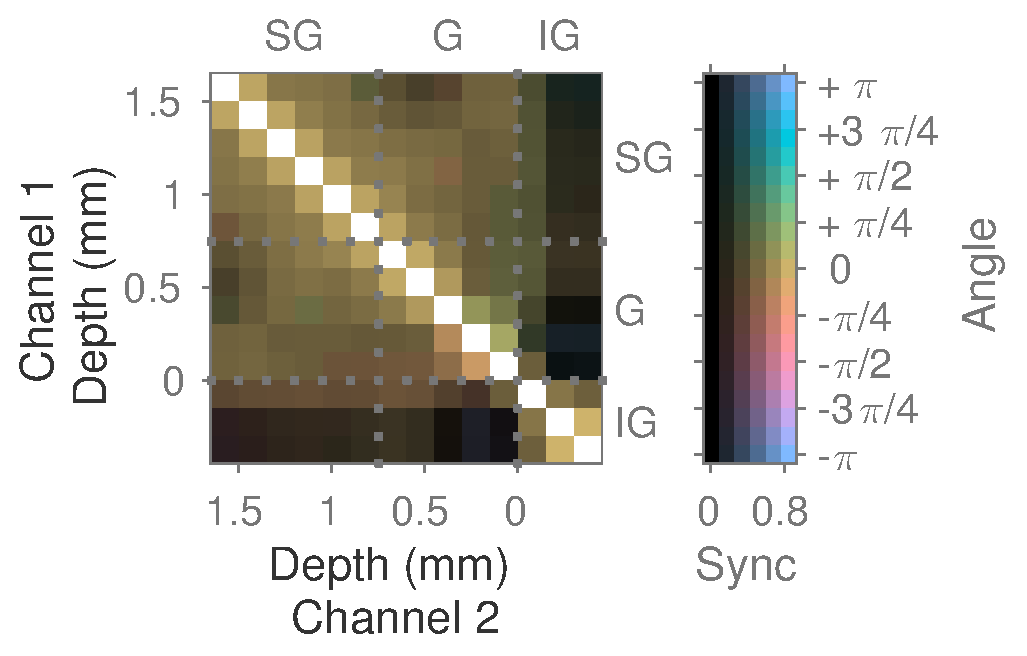
\includegraphics[scale=.45]{phasestats/movie1_Csd_phs4-16_dPhs_combo_5mean.eps}
}
    \\
    \subfloat[Spontaneous.\label{fig:lam_phasestats_alpha_combo_csd_spont}]{
        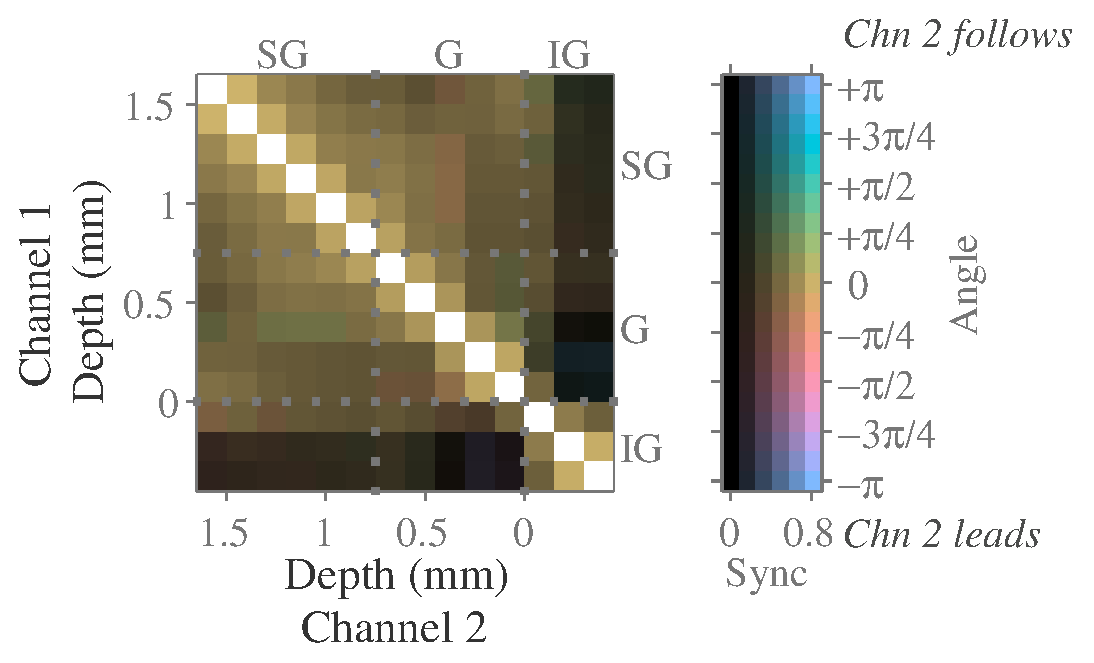
\includegraphics[scale=.45]{phasestats/spont_Csd_phs4-16_dPhs_combo_5mean.eps}
}
    \caption{
\captionemph{\SIrange{4}{16}{Hz} phase synchrony between cortical depths.}
The two-dimensional colour scale shows both average phase offset (hue) and phase synchrony (lightness).
Positive phase differences (green) correspond to the phase of channel 1 ($y$-axis) leading that of channel 2 ($x$-axis).
Negative phase differences (red) correspond to the phase of channel 2 ($x$-axis) leading channel 1 ($y$-axis).
Similar phases are shown in yellow and opposing phases in blue.
The phase synchrony is shown for stimulus driven \protect\subref{fig:lam_phasestats_alpha_combo_csd_movie} and spontaneous \protect\subref{fig:lam_phasestats_alpha_combo_csd_spont} activity.
}
\label{fig:lam_phasestats_alpha_combo_csd}
\end{figure}


% \begin{figure}[htbp]
%     \centering
%     \hspace*{\fill}
%     \subfloat[Movie driven\label{fig:lam_phasestats_alpha_summary_csd_movie}]{
%         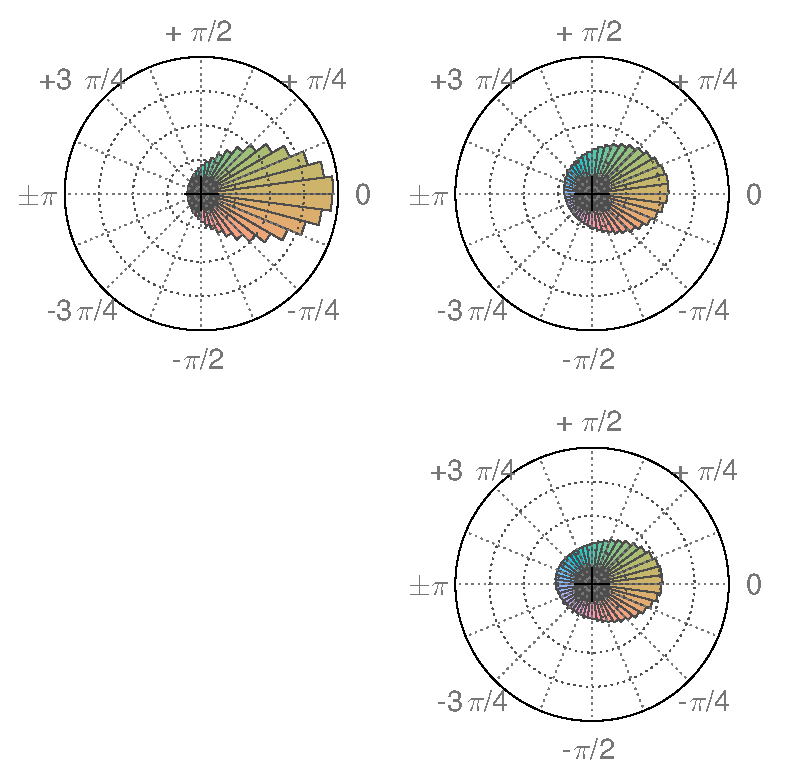
\includegraphics[scale=.45]{phasestats/movie1_Csd_simplephs4-16_dPhs_hist.eps}
% }
%     \hspace*{\fill}\hspace{.2cm}\hspace*{\fill}
%     \subfloat[Spontaneous\label{fig:lam_phasestats_alpha_summary_csd_spont}]{
%         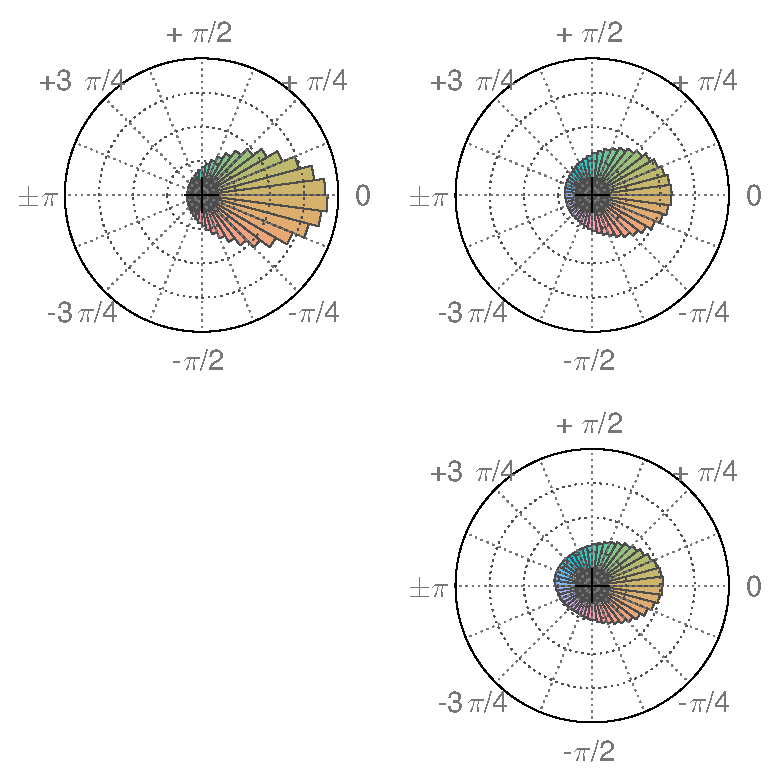
\includegraphics[scale=.45]{phasestats/spont_Csd_simplephs4-16_dPhs_hist.eps}
% }
%     \hspace*{\fill}
%     \caption{Phase correlation, summary by region, \SIrange{4}{16}{Hz}.
% \protect\subref{fig:lam_phasestats_alpha_summary_csd_movie}:~Movie driven.
% \protect\subref{fig:lam_phasestats_alpha_summary_csd_spont}:~Spontaneous.
% }
% \label{fig:lam_phasestats_alpha_summary_csd}
% \end{figure}


%-------------------------------------------------------------------------------
%\FloatBarrier
% \subsubsection{Phase synchrony, \SIrange{60}{170}{Hz}}
%-------------------------------------------------------------------------------

% \begin{figure}[htbp]
%     \centering
%     \hspace*{\fill}
%     \subfloat[Movie driven\label{fig:lam_phasestats_gamma_line_csd_movie}]{
%         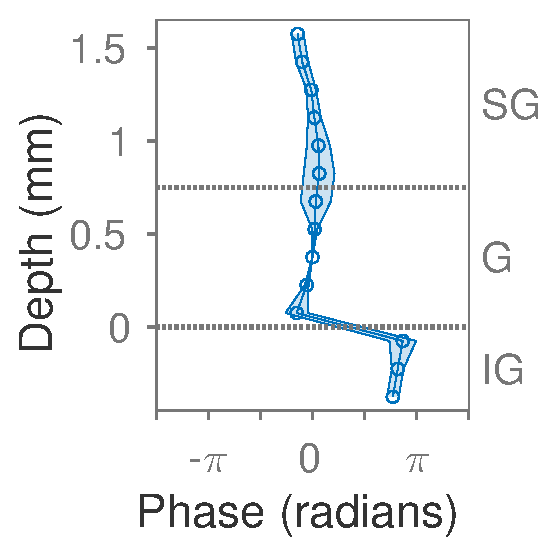
\includegraphics[scale=.45]{phasestats/movie1_Csd_phs60-170_dPhsTracebnd_5mean.eps}
% }
%     \hspace*{\fill}\hspace{.2cm}\hspace*{\fill}
%     \subfloat[Spontaneous\label{fig:lam_phasestats_gamma_line_csd_spont}]{
%         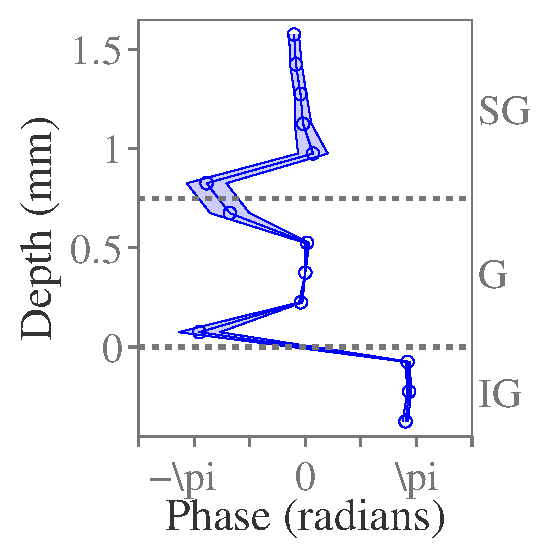
\includegraphics[scale=.45]{phasestats/spont_Csd_phs60-170_dPhsTracebnd_5mean.eps}
% }
%     \hspace*{\fill}
%     \caption{Phase correlation, \SIrange{60}{170}{Hz}.
% \protect\subref{fig:lam_phasestats_gamma_line_csd_movie}:~Movie driven.
% \protect\subref{fig:lam_phasestats_gamma_line_csd_spont}:~Spontaneous.
% }
% \label{fig:lam_phasestats_gamma_line_csd}
% \end{figure}

% \begin{figure}[htbp]
%     \centering
%     \hspace*{\fill}
%     \subfloat[Movie driven\label{fig:lam_phasestats_gamma_hist_csd_movie}]{
%         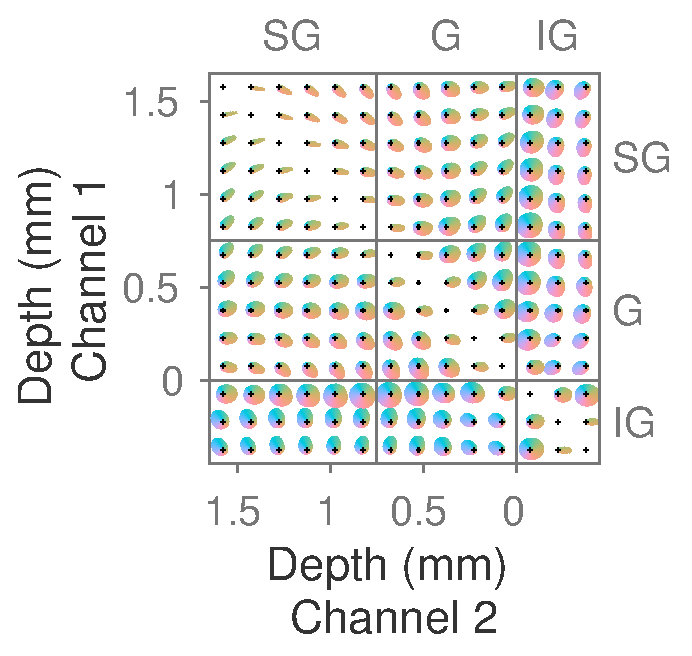
\includegraphics[scale=.45]{phasestats/movie1_Csd_phs60-170_dPhs_hist_5mean.eps}
% }
%     \hspace*{\fill}\hspace{.2cm}\hspace*{\fill}
%     \subfloat[Spontaneous\label{fig:lam_phasestats_gamma_hist_csd_spont}]{
%         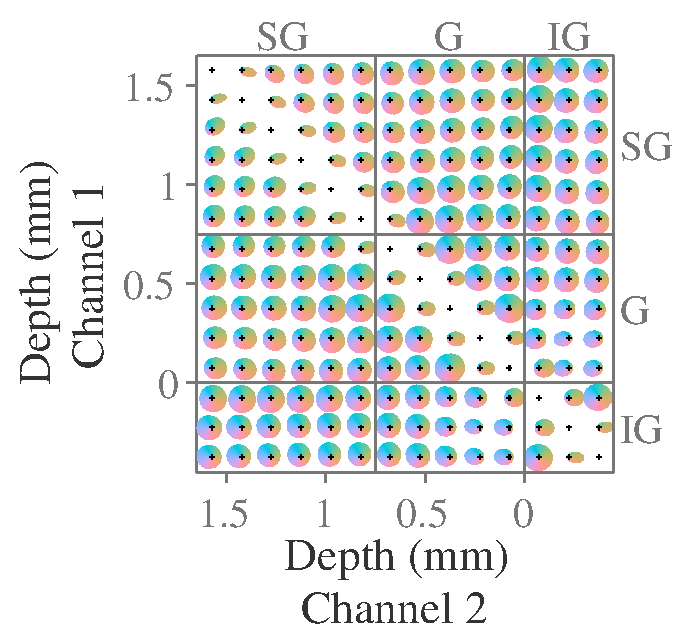
\includegraphics[scale=.45]{phasestats/spont_Csd_phs60-170_dPhs_hist_5mean.eps}
% }
%     \hspace*{\fill}
%     \caption{Phase correlation, \SIrange{60}{170}{Hz}.
% \protect\subref{fig:lam_phasestats_gamma_hist_csd_movie}:~Movie driven.
% \protect\subref{fig:lam_phasestats_gamma_hist_csd_spont}:~Spontaneous.
% }
% \label{fig:lam_phasestats_gamma_hist_csd}
% \end{figure}


We determined the phase difference and synchrony for the \SIrange{60}{170}{Hz} oscillations in the \ac{CSD} in the same manner as for the \SIrange{4}{16}{Hz} frequency range.
As shown in \autoref{fig:lam_phasestats_gamma_combo_csd}, the phase of lower-\ac{G} is typically opposed to that of \ac{IG}.
This may correspond to the source-sink reversal associated with the stimulus onset which we discussed in \autoref{sec:lam_align}.
There is also a gradient in phase across \ac{SG} and \ac{G}, with the middle of \ac{G} leading the response.

We observed there is less synchrony in the spontaneous activity than the stimulus driven activity, but the relationship in the phase across the cortex is the same in both cases.

\begin{figure}[htbp]
    \centering
    \subfloat[Stimulus driven.\label{fig:lam_phasestats_gamma_combo_csd_movie}]{
        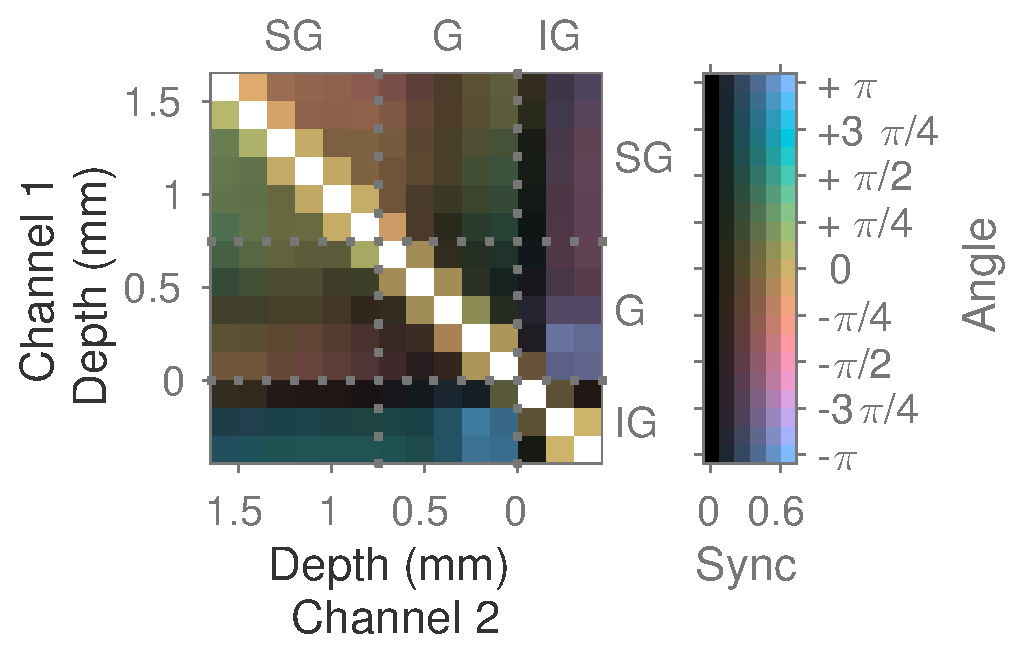
\includegraphics[scale=.45]{phasestats/movie1_Csd_phs60-170_dPhs_combo_5mean.eps}
}
    \\
    \subfloat[Spontaneous.\label{fig:lam_phasestats_gamma_combo_csd_spont}]{
        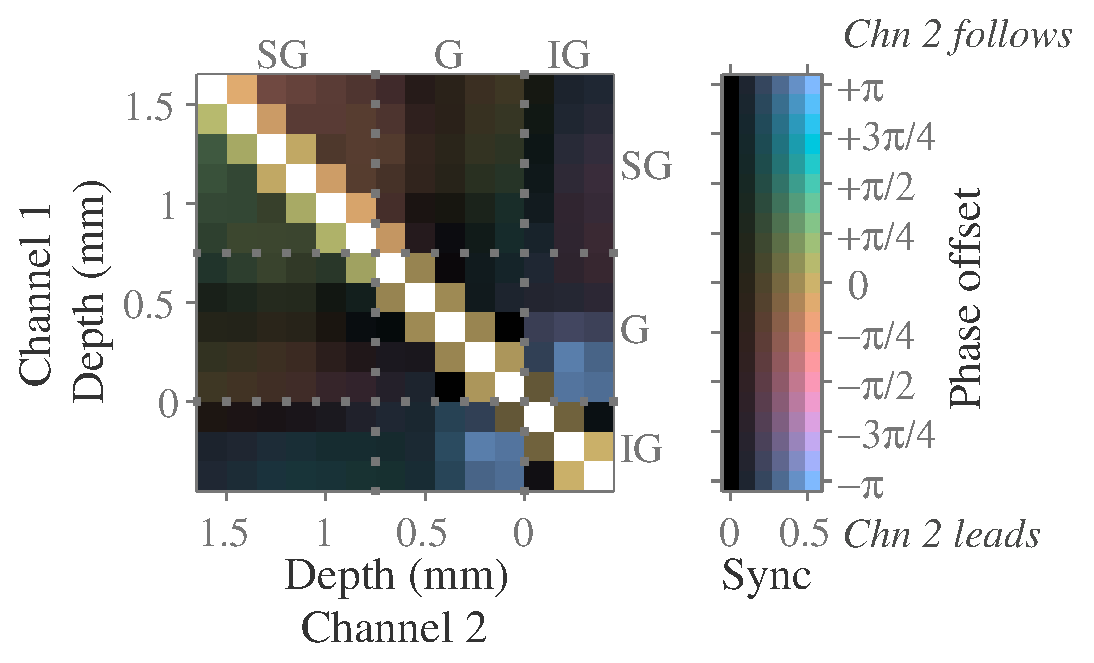
\includegraphics[scale=.45]{phasestats/spont_Csd_phs60-170_dPhs_combo_5mean.eps}
}
\caption{
\captionemph{\SIrange{60}{170}{Hz} phase synchrony between cortical depths.}
The two-dimensional colour scale shows both average phase offset (hue) and phase synchrony (lightness).
Positive phase differences (green) correspond to the phase of channel 1 ($y$-axis) leading that of channel 2 ($x$-axis).
Negative phase differences (red) correspond to the phase of channel 2 ($x$-axis) leading channel 1 ($y$-axis).
Similar phases are shown in yellow and opposing phases in blue.
The phase synchrony is shown for stimulus driven \protect\subref{fig:lam_phasestats_gamma_combo_csd_movie} and spontaneous \protect\subref{fig:lam_phasestats_gamma_combo_csd_spont} activity.
}
\label{fig:lam_phasestats_gamma_combo_csd}
\end{figure}


% \begin{figure}[htbp]
%     \centering
%     \hspace*{\fill}
%     \subfloat[Movie driven\label{fig:lam_phasestats_gamma_summary_csd_movie}]{
%         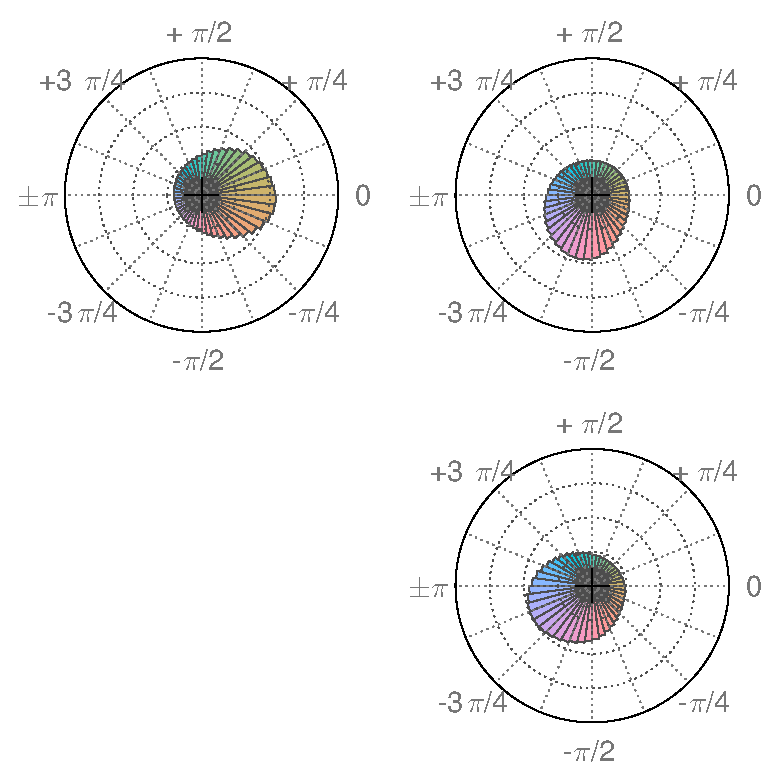
\includegraphics[scale=.45]{phasestats/movie1_Csd_simplephs60-170_dPhs_hist.eps}
% }
%     \hspace*{\fill}\hspace{.2cm}\hspace*{\fill}
%     \subfloat[Spontaneous\label{fig:lam_phasestats_gamma_summary_csd_spont}]{
%         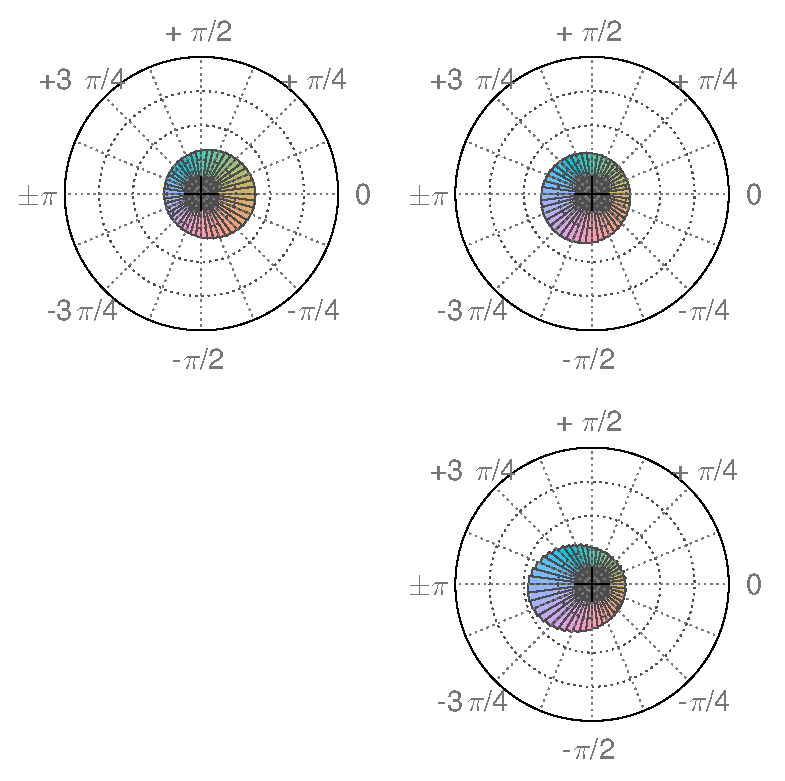
\includegraphics[scale=.45]{phasestats/spont_Csd_simplephs60-170_dPhs_hist.eps}
% }
%     \hspace*{\fill}
%     \caption{Phase correlation, summary by region, \SIrange{60}{170}{Hz}.
% \protect\subref{fig:lam_phasestats_gamma_summary_csd_movie}:~Movie driven.
% \protect\subref{fig:lam_phasestats_gamma_summary_csd_spont}:~Spontaneous.
% }
% \label{fig:lam_phasestats_gamma_summary_csd}
% \end{figure}


%-------------------------------------------------------------------------------
%\FloatBarrier
\subsection{Cross-frequency phase-amplitude coupling}
\label{sec:lam_cfc}
%-------------------------------------------------------------------------------

Another manner in which we can investigate the relationship between phase and power is cross-frequency coupling.
Cross-frequency coupling occurs when the phase of one frequency band is correlated with the envelope amplitude for another frequency band.
To investigated the cross-frequency coupling between the \SIrange{4}{16}{Hz} phase and the \SIrange{60}{170}{Hz} envelope amplitude using the modulation index, described in \autoref{sec:lam_cfc_method}.

\begin{figure}[htbp]
\subfloat{\label{fig:lam_cfc_movie}}
\subfloat{\label{fig:lam_cfc_spont}}
\subfloat{\label{fig:lam_cfc_movie_traces}}
\subfloat{\label{fig:lam_cfc_spont_traces}}
\centering 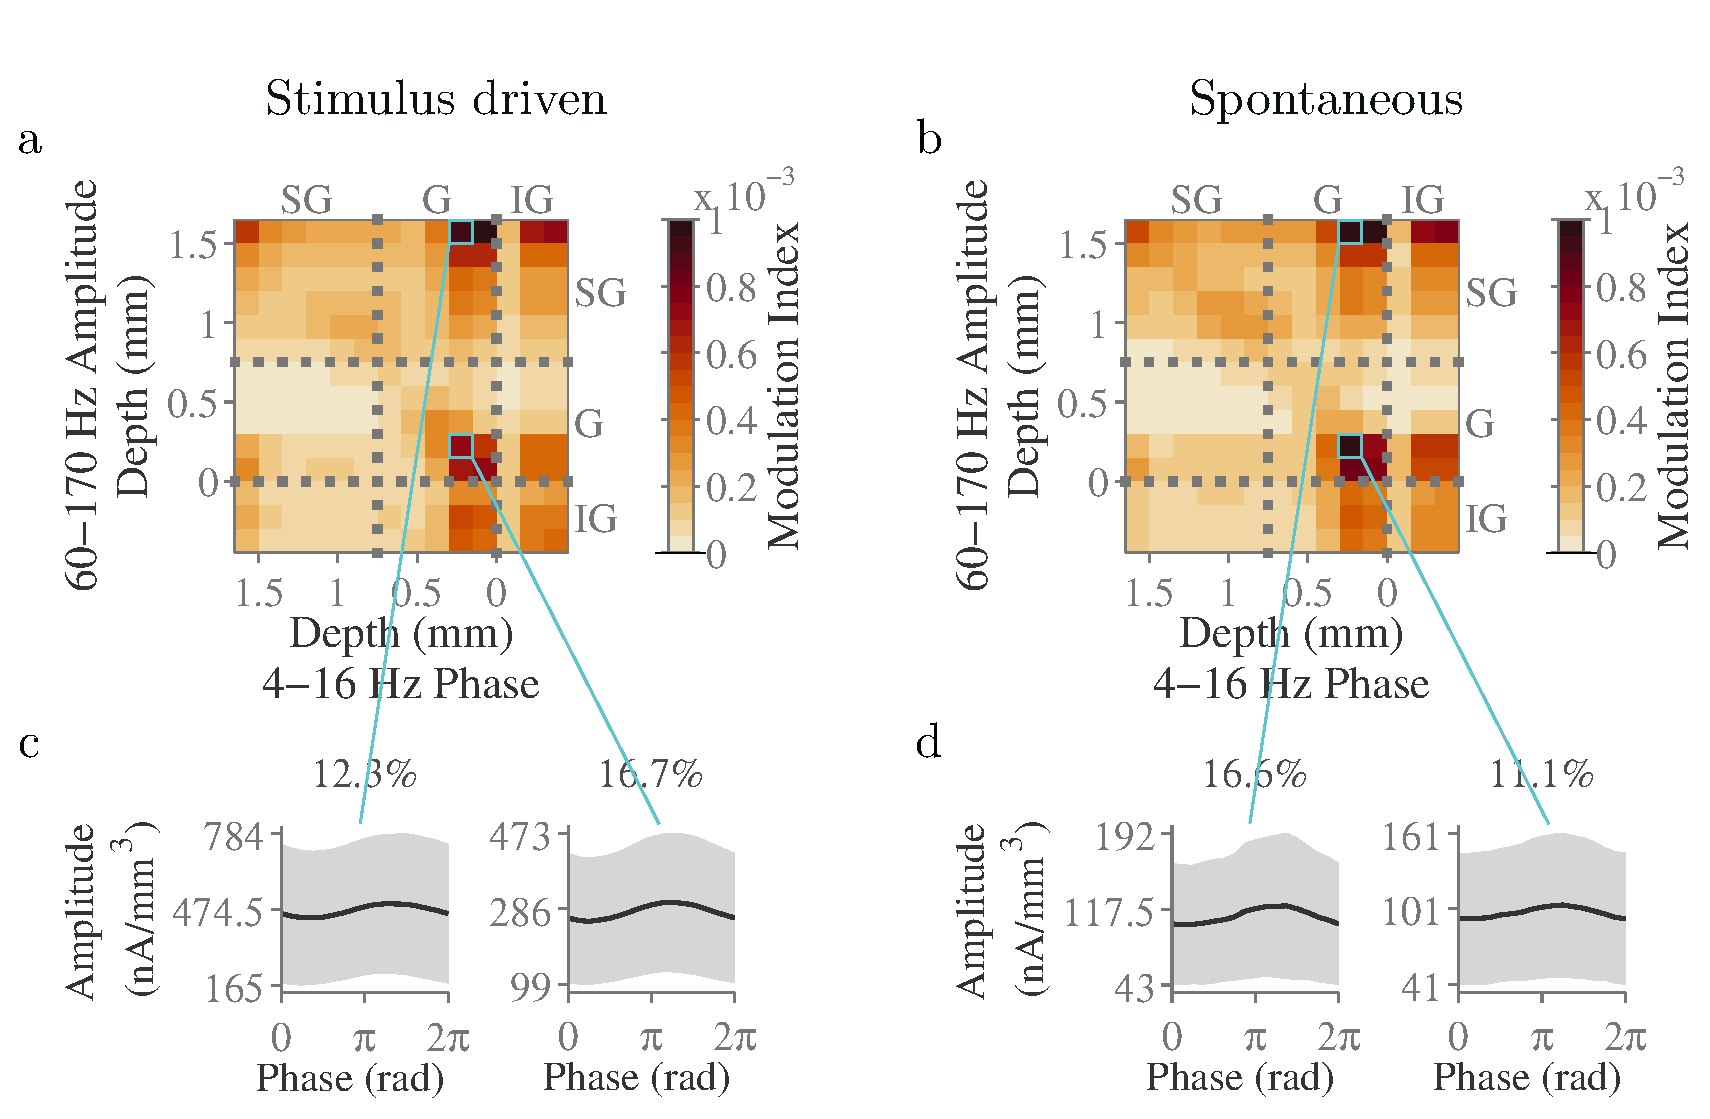
\includegraphics[scale=0.5]{cfc/crossfreqcoupling.eps}
%
\caption{
\captionemph{Cross-frequency phase-amplitude coupling}
Phase-amplitude modulation index between low frequency (\SIrange{4}{16}{Hz}) phase and high frequency (\SIrange{60}{170}{Hz}) amplitude (\protect\subref{fig:lam_cfc_movie}:~movie driven activity; \protect\subref{fig:lam_cfc_spont}:~spontaneous activity).
Mean of \num{5} sessions.
\protect\subref{fig:lam_cfc_movie_traces} and \protect\subref{fig:lam_cfc_spont_traces}:~Amplitude as a function of binned phase for a typical example session (\sesname{F10nm1}), for \ac{IG}$\rightarrow$\ac{IG} coupling (left) and \ac{IG}$\rightarrow$\ac{SG} coupling (right).}%
\label{fig:lam_8}
%
\end{figure}

We observed a spatially localised coupling between the \SIrange{4}{16}{Hz} phase of both lower-\ac{G} and mid-\ac{IG} with the amplitude of \SIrange{60}{170}{Hz} oscillations in upper-\ac{SG} (\autoref{fig:lam_8}).
Additionally, in both \ac{G} and \ac{IG} there is a coupling between the local \SIrange{4}{16}{Hz} phase and the local \SIrange{60}{170}{Hz} amplitude.
The same relationship was discovered to hold both for spontaneous activity and stimulus-driven recordings, and our findings are in agreement with previous work \citep{Spaak2012}.


%-------------------------------------------------------------------------------
\section{Conclusions}
%-------------------------------------------------------------------------------

We considered the amount of information encoded in the phase of cortical oscillations.
For low frequency oscillations (\SI{<40}{Hz}) we found there was around $50\%$ more information in the phase than there was in the power.
Higher frequency oscillations have phases which vary too quickly to reliably correspond to the same parts of the stimulus, and hence we do not find they convey much information about the stimulus.

We found that the information in the phase of any pair of oscillation frequencies less than \SI{40}{Hz} (recorded within the same cortical depth as each other) were synergistic (except for overlapping bands).
Furthermore, we found a substantial amount of information about the timing of scene cuts in the \ac{CSD} phase.
The occurrence of each scene cut produces a stereotypical waveforms in response in the cortex (not shown), similar to the stimulus-onset response shown in \autoref{fig:lam_align_csd}.
Consequently, we believe the synergy between the phase of non-overlapping cortical frequency bands is because maxima and minima of the overall \ac{CSD} occur when all frequencies strike phase $0$ and $\pi$ simultaneously, and these maxima and minima events are repeatably triggered by the stimulus.

Though we found the phase encodes more information about the stimulus than the power, we were not able to relate it to the rate of change of luminance of the movie at any particular spatiotemporal scales
Other than scene transitions, it is still not clear what information about the stimulus is encoded in the phase.

The information in the phase appears to be compartmentalised, with the \ac{SG} and \ac{G} depths (layers 1--4) encoding independent information to \ac{IG} (\acl{L5/6}).
This finding suggests that there are two different cortical oscillations active in this frequency range, driven by different cortical process and, consequently, arising at different depths in the cortical microcircuit.
Our investigation of the phase synchrony across the cortical depth supports this observation, showing that \SIrange{4}{16}{Hz} oscillations across \ac{SG} and \ac{G} have near-simultaneous phase, which is not synchronised with that of \ac{IG}.
However, we did observe that both of these compartmentalised oscillations, sited higher and lower up the cortical depth, are informative about scene transitions in the movie.
Whichever aspects they encode remain unknown.

In agreement with previous work \citep{Spaak2012}, we found there was cross-frequency coupling between the stimulus-encoding power of gamma oscillations in \acs{L1} and the phase of alpha oscillations in lower \acs{L4}.
Anatomically, we believe this is related to the pyramidal cell bodies in \acs{L5A}, which have apical dendritic tufts in \acs{L1} \citep{Hill2013,Zhu2004}.
This cross-frequency coupling could be one mechanism through which the \acs{L1} gamma oscillations containing high levels of information about the stimulus is converted into an alpha oscillation for feedback into a hierarchically lower cortical region.
Such a mechanism would be support the feedback/feedforward hypothesis of \citet{VanKerkoerle2014} which we discussed in \autoref{sec:lam_discussion}.
However, the direction of causality for the cross-frequency coupling is unknown, so the observed results could instead be manifested by alpha oscillations in \acs{L4} modulating the gamma power in \acs{L1}.
Neurons in \acs{L5} are known to be related to long-range cortical output \citep{Hill2013}, and inputs into \acs{L1} are known to be predominantly inputs from higher-order cortices, so this cross-frequency coupling may provide a system for low-frequency feedback to be translated into higher frequency oscillations within \ac{V1}.
